% !TEX --enable-write18
\documentclass[12pt,a4paper]{report}
%%%%%%%%%%%%%%%%%%%%%%%%%%%%%%%%%%%%%%%%%%%%%%%%%%%%%%%%%%%%%%%
%%%%%%%%%%%%%all_packages%%%%%%%%%%%%%%%%%%%%%%%%%%%%%%%%%%%%%%
\usepackage[T1]{fontenc}
\usepackage{lmodern} % needed on MikTeX
\usepackage[utf8]{inputenc}
\usepackage{imakeidx}
\usepackage[toc]{glossaries}
\usepackage[a4paper,portrait,margin=1in,headheight=15pt]{geometry}
\usepackage{graphicx}
\usepackage{appendix}
\usepackage{caption}
\usepackage{subcaption}
\usepackage{titlesec}
\usepackage{siunitx}
\usepackage[hidelinks,pdfa,pdfusetitle]{hyperref}
\usepackage{array}
\usepackage{float}
\usepackage{fancyhdr}
\usepackage{longtable}
\usepackage{siunitx}
\usepackage{enumitem}
\usepackage{ulem}
\usepackage{multirow}
\usepackage{afterpage}
\usepackage{rotating}
\usepackage{acronym}
\usepackage{tfrupee}  
\usepackage{etoolbox}
\usepackage{listings}
\usepackage[abspage,user,lastpage]{zref}
\usepackage[hang]{footmisc}       %for aligning footnote
\usepackage[backend=biber,refsection=section,sorting=none,style=numeric, defernumbers=true,safeinputenc]{biblatex}
\makeindex[columns = 2, title = AlphabeticalIndex, intoc, options =-s indcomma]
%%%%%%%%%%%%%%%%%%%%%%%%%%%%%%%%%%%%%%%%%%%%%%%%%%%%%%%%%%%%%%%
%%%%%%%%%%%%%%%%%%%%%%%%%%%%%%%%%%%%%%%%%%%%%%%%%%%%%%%%%%%%%%%
%%%%%%%%%%%%%%%%%%%preamble and packages for first page%%%%%%%%%%%%%%%%%%%%%%%%%
\usepackage[dvipsnames, svgnames]{xcolor}
\usepackage{tikz}
\usepackage{xspace}
\usepackage{pdfpages}
\usepackage{afterpage}
\usepackage{graphicx}
\usepackage{hyperxmp}
\usepackage{url}
\urlstyle{sf}
\usepackage{ccicons} % use Creative Commons icons
\usepackage[absolute]{textpos} % exact position logo
\usepackage{amsmath} % https://ctan.org/pkg/amsmath for mathematical features
\makeindex[columns = 2, title = Alphabetical Index, intoc, options =-s indcomma]

%% Fonts and typography
%\usepackage{helvet}           
\usepackage[scaled=0.95]{helvet} % Helvetica (kerning adjusted)
\renewcommand{\sfdefault}{phv}     % Helvetica
\usepackage[final]{microtype}  % Improved typography

\definecolor{tuberlingrayarea}{RGB}{249 247 247} % gray #F9F7F7 for background
\definecolor{tuberlindarkgray}{RGB}{91 75 75} % gray #5B4B4B for headings
%%%%%%%%%%%%%%%%%%%%%%%%%%%%%%%%%%%%%%%%%%%%%%%%%%%%%%%%%%%%%%%%%%%%%%%%%%%%%%%%%%%%%%

% to remove the chapter word in the pages
\titleformat{\chapter}[display]
{\normalfont\bfseries}{}{0pt}{\Huge}

% The following definition is copied from authortitle.bbx/authoryear.bbx
\defbibenvironment{nolabelbib}
  {\list
     {}
     {\setlength{\leftmargin}{\bibhang}%
      \setlength{\itemindent}{-\leftmargin}%
      \setlength{\itemsep}{\bibitemsep}%
      \setlength{\parsep}{\bibparsep}}}
  {\endlist}
  {\item}


% adding bibliography sources
\addbibresource{Files/Chapters/Appendices/references.bib}
\nocite{*}

% Page style
\pagestyle{fancy}
\fancyhf{}
\fancyhead[R]{\thepage}
\fancyhead[L]{\nouppercase{\leftmark}}

%footnote style
\setlength\footnotemargin{10pt}
\makenoidxglossaries
\renewcommand{\glsnamefont}[1]{\makefirstuc{#1}}

\newglossaryentry{6/6 vision}{
    name=6/6 vision,
    description={denotes normal eyesight, where an individual can see details from a distance of 6 meters equivalent to what a person with typical vision sees at the same distance}
}
\newglossaryentry{$24$-hour clock}{
    name=$24$-hour clock,
    description={It is a timekeeping system where the hours beyond 12:00 are expressed without the use of AM or PM indicators.}
}
\newglossaryentry{accelerometer}{
    name=accelerometer,
    description={An instrument for measuring the acceleration of a body, which in practical terms means changes in speed or direction of a motion.}
}
\newglossaryentry{audio unit}{
    name=audio unit,
    description={Provides audio announcements using speakers regarding the estimated arrival time of the bus at specific bus stops.}
}
\newglossaryentry{DC/DC converter}{
    name=DC/DC converter,
    description={A DC-DC converter is an electronic circuit or electromechanical device that converts a source of direct current from one voltage level to another.}
}
\newglossaryentry{embedded system}{
    name=Embedded system,
    description={An embedded system is a specialized computer system designed to perform specific tasks within a larger system or device.}
}
\newglossaryentry{GPS}{
    name=GPS,
    description={GPS stands for Global Positioning System. It is a satellite-based navigation system that enables users to determine their precise location anywhere on Earth.}
}
\newglossaryentry{LED dot matrix display}{
    name=LED dot matrix display,
    description={A grid of light-emitting diodes (LEDs) arranged in rows and columns, allowing each LED to be individually controlled to display characters by selectively turning on or off specific LEDs in the matrix.}
}
\newglossaryentry{MPPT converter}{
    name=MPPT converter,
    description={Stands for  Maximum Power Point Tracking , it is a type of DC/DC converter commonly used in photovoltaic systems to optimize the power output of solar panels by continuously adjusting the operating point to maximize energy harvest from the panels.}
}
\newglossaryentry{PWM converter}{
    name=PWM converter,
    description={A type of power electronics device used to regulate the output voltage or current by controlling the duty cycle of a pulse-width modulated signal.}
}
\newglossaryentry{round trip}{
    name=round trip,
    description={Refers to a journey where a bus travels from a starting point to a destination and then returns back to the original starting point.}
}
\newglossaryentry{smog}{
    name=smog,
    description={A type of air pollution that consists of a mixture of smoke and fog, often caused by industrial emissions, vehicle exhaust, and atmospheric conditions.}
}
\newglossaryentry{sliding text animation}{
    name=sliding text animation,
    description={It is a visual effect over a display where text moves smoothly across the screen horizontally, vertically, or diagonally.}
}
\newglossaryentry{stall period}{
    name=stall period,
    description={Refers to a duration of time during which the system pauses temporarily until the situation is resolved, allowing the system to resume its intended function.}
}
\newglossaryentry{USB}{
    name=USB,
    description={Stands for Universal Serial Bus. It is a standardized interface commonly used for connecting peripherals to computers and other electronic devices.}
}
\newglossaryentry{ultrasonic sensor}{
    name=ultrasonic sensor,
    description={A device that utilizes ultrasonic waves, typically operating in the frequency range of 20 kHz to 200 kHz, to detect the presence and distance objects by emitting ultrasonic pulses and measuring the time it takes for the pulses to reflect back from objects.}
}
\newglossaryentry{U-turn}{
    name=U-turn,
    description={When a vehicle turns 180 degrees to reverse its direction and proceed in the opposite direction.}
}
\newglossaryentry{Wi-Fi}{
    name=Wi-Fi,
    description={Wireless Fidelity, is a technology that allows electronic devices to connect to the internet or communicate with one another wirelessly using radio frequencies.}
}


%defining new alignment
\newcolumntype{n}{>{\centering} m{5.5cm}}
\newcolumntype{e}{>{\raggedleft} m{3.1cm}}
\newcolumntype{E}{>{\raggedleft} m{5.1cm}}


%%%%%%%%%%%%%%%%%%%%%%%%%%%%%%%%%%%%%%%%%%%%%%%%%%%%%%%%%%%%%%%%%
%%%             Landscape Environment                         %%%
%%%        (Must load etoolbox package before)                %%%
%%%    And use /savegeometry before the using landscape page  %%%
%%%      and use /loadgeometry after the landscape page       %%%
%%%%%%%%%%%%%%%%%%%%%%%%%%%%%%%%%%%%%%%%%%%%%%%%%%%%%%%%%%%%%%%%%

\makeatletter
 \def\ifGm@preamble#1{\@firstofone}
  \appto\restoregeometry{%
     \pdfpagewidth=\paperwidth
     \pdfpageheight=\paperheight}
 \apptocmd\newgeometry{%
    \pdfpagewidth=\paperwidth
    \pdfpageheight=\paperheight}{}{}
 \makeatother


\newenvironment{landscapes}{
    \newpage
    \newgeometry{margin=1in,landscape}  
}{%
\newpage
}

\fancypagestyle{uselscape}{
	\fancyhf{}
	\fancyhead[R]{\thepage}
	\fancyhead[L]{\nouppercase{\rightmark}}
	\fancyheadoffset[R]{0mm}
	}

%%%%%%%%%%%%%%%%%%%%%%%% Start of Document %%%%%%%%%%%%%%%%%%%%

\begin{document}
\renewcommand{\thefootnote}{\alph{footnote}}
\begin{titlepage}
    \newgeometry{voffset=-1in,textwidth=160mm, textheight=253mm,margin=1in}
   % \newgeometry{hoffset=-1in, voffset=-1in, textwidth=160mm, textheight=253mm, topmargin=22mm, headsep=0mm, headheight=0mm, lmargin=2.2in, marginparpush=0mm,footheight=0mm, footsep=0mm}

    % Logo right corner - change to black-white if needed
       \begin{textblock*}{6cm}(14cm,4cm)
       
\includegraphics[width=2in]{Files/Images/iitdlogo.png}
       %\includegraphics[width=50mm]{def/TU_Logo_lang_RGB_schwarz.pdf}
       \end{textblock*}
         %%% gray background
            \vskip1in
            \begin{tikzpicture}[remember picture, overlay]         
	        \fill [tuberlingrayarea, opacity=1] (-1.2,-7.0) rectangle (16,-26);
	        \end{tikzpicture}
	        \raggedright
            \vskip3in
             %%% title elements
              {%
				\fontsize{20}{28}
				\boldmath
				\sffamily
				 Tribe: CleanTeX
				\par
            }
             \vskip0.25in
           
             {
				\Large
				\fontsize{28}{32}
				\bfseries
				\boldmath
				\sffamily
                Bus Stand Display Unit
				\par
            }
            \vskip0.15in
             {
				\fontsize{18}{18}
				\sffamily
                
				\par
            }
            \vskip0.15in
             {
				\fontsize{16}{16}
				\sffamily
                ELP305 : Design and System Laboratory
				\par
            }
            \vskip0.15in
             {
				\fontsize{16}{14}
				\sffamily
                \textbf{Indian Institute of Technology, Delhi}
                \par
            }
    \vspace{0.5in}
    {
        \normalsize
        %\fontsize{10}{12}
        \sffamily
        \textbf{\textcolor{tuberlindarkgray}{Document Authorised by}}\par \vspace{0.125cm}
        {\href{https://www.linkedin.com/in/ayush-gupta-undergraduate/}{Ayush Gupta}, \href{http://linkedin.com/in/aryan-mishra-04j}{Aryan Mishra}}

        \vspace{0.25cm}
        \textbf{\textcolor{tuberlindarkgray}{Release Date}}\par \vspace{0.125cm}
        {\today}

        \vspace{0.25cm}
        \textbf{\textcolor{tuberlindarkgray}{Release Version}}\par \vspace{0.125cm}
        \textbf{v0.2.13
}\footnote{Tracked automatically in the \textbf{GitHub} Repository.
                  \textbf{v0.0.1} was the first release after P2 release on March 13, 2024.
                  Version number is stepped up, based on whether it is a \textbf{Minor Release} or a \textbf{Bug Fix}.
                  The file after submission at the end of each week is considered a \textbf{Major Release}.}

        \vspace{0.25cm}
        \textbf{\textcolor{tuberlindarkgray}{Release Type}}\par \vspace{0.125cm}
        {Private Release}

        \vspace{0.25cm}
        \textbf{\textcolor{tuberlindarkgray}{Terms Of Use}}\par \vspace{0.125cm}
        {All Rights Reserved}

        \vspace{0.25cm}
        \textbf{\textcolor{tuberlindarkgray}{Project Details}}\par \vspace{0.125cm}
        {This project is being managed on \href{https://github.com/ELP305-Cleaning-Machine}{GitHub} and the latest version of this report is hosted \href{https://2nav.github.io/TribeC/}{here}.}
    }
\end{titlepage}
\afterpage{\restoregeometry}    

\pagenumbering{roman}
\tableofcontents
\pagestyle{fancy}
\chapter{Introduction}

\section{Overall Coordinators}
    \begin{center}
	    \label{table:oc}
	    \begin{longtable}{ | n | e | E | c| }
		    \hline
		    \textbf{Name}                                                                & \textbf{Entry Number} & \textbf{Email ID}                                                    & \textbf{IF} \\
		    \hline \hline\href{http://linkedin.com/in/aryan-mishra-04j}{Aryan Mishra} & 2021EE10137 & \href{mailto:ee1210137@ee.iitd.ac.in}{ee1210137@ee.iitd.ac.in} & 1.0\\ 
\hline 
\href{https://www.linkedin.com/in/ayush-gupta-undergraduate/}{Ayush Gupta} & 2021MT10697 & \href{mailto:mt1210697@maths.iitd.ac.in}{mt1210697@maths.iitd.ac.in} & 1.0\\ 
\hline 

		    \caption{Overall Coordinators}
	    \end{longtable}
    \end{center}
    \section{Subtribes\footnote{\textbf{\textit{Activity Coordinator} written in bold}}}
    \subsection{Documentation}
    \begin{center}
    \label{table:Docu1}
    \begin{longtable}{| n | e | E | c| }
        \hline
        \textbf{Name}                                                                                                      & \textbf{Entry Number} & \textbf{Email ID}                                                    & \textbf{IF} \\
        \hline \hline\href{https://its-archisman.github.io/My-Website/}{\textbf{Archisman Biswas} } & 2021MT10254 & \href{mailto:mt1210254@maths.iitd.ac.in}{mt1210254@maths.iitd.ac.in} & 1.0\\ 
\hline 
\href{https://github.com/Azm1t}{Asmit Singh} & 2021MT10887 & \href{mailto:mt1210887@maths.iitd.ac.in}{mt1210887@maths.iitd.ac.in} & 1.0\\ 
\hline 
\href{https://github.com/Musaibgani}{Musaib Gani Pirzada} & 2021MT10227 & \href{mailto:mt1210227@maths.iitd.ac.in}{mt1210227@maths.iitd.ac.in} & 0.98\\ 
\hline 
\href{github.com/2nav}{Navneet Raj} & 2021MT10240 & \href{mailto:mt1210240@maths.iitd.ac.in}{mt1210240@maths.iitd.ac.in} & 1.0\\ 
\hline 
\href{Alice-Mina}{Neelam Kumari Meena} & 2021MT10938 & \href{mailto:mt1210938@maths.iitd.ac.in}{mt1210938@maths.iitd.ac.in} & 0.95\\ 
\hline 
\href{nan}{Nikhil Choudhary} & 2020MT10826 & \href{mailto:mt1200826@maths.iitd.ac.in}{mt1200826@maths.iitd.ac.in} & 0.9\\ 
\hline 
\href{https://www.linkedin.com/in/purushottam-malviya-9225681bb/}{Purushottam Malviya} & 2020EE10531 & \href{mailto:ee1200531@ee.iitd.ac.in}{ee1200531@ee.iitd.ac.in} & 0.95\\ 
\hline 
\href{https://www.linkedin.com/in/rahul-bhardwaj-dintyala-244117202/}{Rahul Bhardwaj} & 2020MT60877 & \href{mailto:mt6200877@maths.iitd.ac.in}{mt6200877@maths.iitd.ac.in} & 1.0\\ 
\hline 
\href{nan}{Rishabh Barola} & 2021EE10636 & \href{mailto:ee1210636@ee.iitd.ac.in}{ee1210636@ee.iitd.ac.in} & 1.0\\ 
\hline 
\href{nan}{Saket Kandoi} & 2021MT60265 & \href{mailto:mt6210265@maths.iitd.ac.in}{mt6210265@maths.iitd.ac.in} & 0.9\\ 
\hline 
\href{https://github.com/Sanjay23Pooniya}{Sanjay Pooniya} & 2021EE10148 & \href{mailto:ee1210148@ee.iitd.ac.in}{ee1210148@ee.iitd.ac.in} & 1.0\\ 
\hline 
\href{https://www.linkedin.com/in/sanskriti-gautam-1161b6236/}{Sanskriti Gautam} & 2021MT10935 & \href{mailto:mt1210935@maths.iitd.ac.in}{mt1210935@maths.iitd.ac.in} & 1.0\\ 
\hline 
\href{https://iamsecretlyflash.github.io/}{Vaibhav Seth} & 2021MT10236 & \href{mailto:mt1210236@maths.iitd.ac.in}{mt1210236@maths.iitd.ac.in} & 0.95\\ 
\hline 
\href{https://github.com/crownCTDM}{Vasu Sharma} & 2021EE10620 & \href{mailto:ee1210620@ee.iitd.ac.in}{ee1210620@ee.iitd.ac.in} & 0.85\\ 
\hline 
\hline
		    \caption{Documentation}
	    \end{longtable}
    \end{center}
    \subsection{Others}
    \begin{center}
    \label{table:Othe1}
    \begin{longtable}{| n | e | E | c| }
        \hline
        \textbf{Name}                                                                                                      & \textbf{Entry Number} & \textbf{Email ID}                                                    & \textbf{IF} \\
        \hline \hline\href{https://github.com/Hello-3585}{Abhinav Verma} & 2021EE10978 & \href{mailto:ee1210978@ee.iitd.ac.in}{ee1210978@ee.iitd.ac.in} & 1.0\\ 
\hline 
\href{4-tohchalega}{Aditya Jain} & 2021EE10633 & \href{mailto:ee1210633@ee.iitd.ac.in}{ee1210633@ee.iitd.ac.in} & 0.68\\ 
\hline 
\href{https://github.com/Ameya-Mishra}{Ameya Mishra} & 2021MT10637 & \href{mailto:mt1210637@maths.iitd.ac.in}{mt1210637@maths.iitd.ac.in} & 0.68\\ 
\hline 
\href{https://www.linkedin.com/in/anchal-popli-182047225/}{Anchal} & 2021MT10910 & \href{mailto:mt1210910@maths.iitd.ac.in}{mt1210910@maths.iitd.ac.in} & 0.86\\ 
\hline 
\href{https://www.linkedin.com/in/aniket-abhiraj-357381237/}{Aniket Abhiraj} & 2021EE10676 & \href{mailto:ee1210676@ee.iitd.ac.in}{ee1210676@ee.iitd.ac.in} & 0.98\\ 
\hline 
\href{lunatic04}{Aniket Singh} & 2021MT10256 & \href{mailto:mt1210256@maths.iitd.ac.in}{mt1210256@maths.iitd.ac.in} & 0.68\\ 
\hline 
\href{https://github.com/Anshulydav}{Anshul} & 2021EE10729 & \href{mailto:ee1210729@ee.iitd.ac.in}{ee1210729@ee.iitd.ac.in} & 1.0\\ 
\hline 
\href{nan}{Ark Verma} & 2021EE10783 & \href{mailto:ee1210783@ee.iitd.ac.in}{ee1210783@ee.iitd.ac.in} & 0.88\\ 
\hline 
\href{https://github.com/ArnavGoel458}{Arnav Goel} & 2021EE10699 & \href{mailto:ee1210699@ee.iitd.ac.in}{ee1210699@ee.iitd.ac.in} & 0.68\\ 
\hline 
\href{https://www.linkedin.com/in/aryan-gupta-43b283229}{Aryan Gupta} & 2021EE10974 & \href{mailto:ee1210974@ee.iitd.ac.in}{ee1210974@ee.iitd.ac.in} & 1.0\\ 
\hline 
\href{https://github.com/Dhruv-Kushwaha2010}{Dhruv Kushwaha} & 2021MT10235 & \href{mailto:mt1210235@maths.iitd.ac.in}{mt1210235@maths.iitd.ac.in} & 0.88\\ 
\hline 
\href{https://github.com/Harsh2718}{Harsh Agarwal} & 2021EE30977 & \href{mailto:ee3210977@ee.iitd.ac.in}{ee3210977@ee.iitd.ac.in} & 1.0\\ 
\hline 
\href{https://github.com/harshswaika}{Harsh Swaika} & 2021EE11052 & \href{mailto:ee1211052@ee.iitd.ac.in}{ee1211052@ee.iitd.ac.in} & 0.7\\ 
\hline 
\href{https://github.com/HarshitSachdeva03}{Harshit Sachdeva} & 2021EE30705 & \href{mailto:ee3210705@ee.iitd.ac.in}{ee3210705@ee.iitd.ac.in} & 0.68\\ 
\hline 
\href{https://github.com/wm0395/}{Harshit Singh} & 2021MT10257 & \href{mailto:mt1210257@maths.iitd.ac.in}{mt1210257@maths.iitd.ac.in} & 0.86\\ 
\hline 
\href{nan}{Kaustubh Dev} & 2021EE10689 & \href{mailto:ee1210689@ee.iitd.ac.in}{ee1210689@ee.iitd.ac.in} & 0.92\\ 
\hline 
\href{https://www.linkedin.com/in/khushika-shringi-205419226}{Khushika Shringi} & 2021EE10665 & \href{mailto:ee1210665@ee.iitd.ac.in}{ee1210665@ee.iitd.ac.in} & 1.0\\ 
\hline 
\href{https://www.linkedin.com/in/khushvind-maurya/}{Khushvind Maurya} & 2021MT10238 & \href{mailto:mt1210238@maths.iitd.ac.in}{mt1210238@maths.iitd.ac.in} & 0.68\\ 
\hline 
\href{https://github.com/Kinjal001}{Kinjal Anchhara} & 2021MT60959 & \href{mailto:mt6210959@maths.iitd.ac.in}{mt6210959@maths.iitd.ac.in} & 1.0\\ 
\hline 
\href{https://github.com/maithilij2003}{Maithili Joshi} & 2021EE10653 & \href{mailto:ee1210653@ee.iitd.ac.in}{ee1210653@ee.iitd.ac.in} & 0.98\\ 
\hline 
\href{https://github.com/Mohitraj227}{Mohit Raj Modi} & 2021MT10919 & \href{mailto:mt1210919@maths.iitd.ac.in}{mt1210919@maths.iitd.ac.in} & 0.85\\ 
\hline 
\href{https://www.linkedin.com/in/mridulahi/}{Mridul Ahi} & 2021MT10901 & \href{mailto:mt1210901@maths.iitd.ac.in}{mt1210901@maths.iitd.ac.in} & 0.7\\ 
\hline 
\href{nan}{Namay Bedi Verma} & 2021MT61051 & \href{mailto:mt6211051@maths.iitd.ac.in}{mt6211051@maths.iitd.ac.in} & 0.83\\ 
\hline 
\href{oshink}{Oshin Kavdia} & 2021EE10654 & \href{mailto:ee1210654@ee.iitd.ac.in}{ee1210654@ee.iitd.ac.in} & 0.7\\ 
\hline 
\href{https://www.linkedin.com/in/rohandas1710/}{Rohan Das} & 2021EE10621 & \href{mailto:ee1210621@ee.iitd.ac.in}{ee1210621@ee.iitd.ac.in} & 0.98\\ 
\hline 
\href{nan}{Sai Raj Kolisetti} & 2021EE10145 & \href{mailto:ee1210145@ee.iitd.ac.in}{ee1210145@ee.iitd.ac.in} & 1.0\\ 
\hline 
\href{https://www.linkedin.com/in/sarthak-kumar-singh-a77146245/}{Sarthak Kumar Singh} & 2021EE10673 & \href{mailto:ee1210673@ee.iitd.ac.in}{ee1210673@ee.iitd.ac.in} & 0.98\\ 
\hline 
\href{https://in.linkedin.com/in/shubh-chhabra-007197227}{Shubh Chhabra} & 2021EE10645 & \href{mailto:ee1210645@ee.iitd.ac.in}{ee1210645@ee.iitd.ac.in} & 1.0\\ 
\hline 
\href{aggarwalshubham009}{Shubham Aggarwal} & 2021EE10809 & \href{mailto:ee1210809@ee.iitd.ac.in}{ee1210809@ee.iitd.ac.in} & 1.0\\ 
\hline 
\href{https://www.linkedin.com/in/ujjwal-yadav-880448223}{Ujjwal Yadav} & 2021EE10669 & \href{mailto:ee1210669@ee.iitd.ac.in}{ee1210669@ee.iitd.ac.in} & 0.98\\ 
\hline 
\href{Vishal-495}{Vishal Sai Bingi} & 2021EE10668 & \href{mailto:ee1210668@ee.iitd.ac.in}{ee1210668@ee.iitd.ac.in} & 0.7\\ 
\hline 
\href{https://www.linkedin.com/in/yash-goel-6ba26322}{Yash Goel} & 2021EE10984 & \href{mailto:ee1210984@ee.iitd.ac.in}{ee1210984@ee.iitd.ac.in} & 1.0\\ 
\hline 
\href{https://www.linkedin.com/in/abhilasa-das-194413236}{Abhilasa Das} & 2021EE10168 & \href{mailto:ee1210168@ee.iitd.ac.in}{ee1210168@ee.iitd.ac.in} & 1.0\\ 
\hline 
\href{https://github.com/Aditi188}{Aditi Shekhar} & 2021EE10685 & \href{mailto:ee1210685@ee.iitd.ac.in}{ee1210685@ee.iitd.ac.in} & 1.0\\ 
\hline 
\href{https://www.linkedin.com/in/advait-ninawe-7a790022}{Advait Rajesh Ninawe} & 2021EE30714 & \href{mailto:ee3210714@ee.iitd.ac.in}{ee3210714@ee.iitd.ac.in} & 1.0\\ 
\hline 
\href{https://github.com/AyushKumar284}{Ayush Kumar} & 2021EE10150 & \href{mailto:ee1210150@ee.iitd.ac.in}{ee1210150@ee.iitd.ac.in} & 1.0\\ 
\hline 
\href{https://www.linkedin.com/in/chetan-chaurasia-561b3b228}{Chetan Chaurasia} & 2021EE10147 & \href{mailto:ee1210147@ee.iitd.ac.in}{ee1210147@ee.iitd.ac.in} & 0.7\\ 
\hline 
\href{nan}{Chirag Gautam} & 2021EE10166 & \href{mailto:ee1210166@ee.iitd.ac.in}{ee1210166@ee.iitd.ac.in} & 0.7\\ 
\hline 
\href{nan}{Deepanshu Kumar} & 2021EE10696 & \href{mailto:ee1210696@ee.iitd.ac.in}{ee1210696@ee.iitd.ac.in} & 0.4\\ 
\hline 
\href{lost-strings}{Disha Katia} & 2021EE10647 & \href{mailto:ee1210647@ee.iitd.ac.in}{ee1210647@ee.iitd.ac.in} & 1.0\\ 
\hline 
\href{dn09-create}{Durgesh Nandini} & 2021EE10651 & \href{mailto:ee1210651@ee.iitd.ac.in}{ee1210651@ee.iitd.ac.in} & 1.0\\ 
\hline 
\href{https://github.com/vulpeex}{Eepsita} & 2021EE10692 & \href{mailto:ee1210692@ee.iitd.ac.in}{ee1210692@ee.iitd.ac.in} & 1.0\\ 
\hline 
\href{nan}{Garvit Dhoot} & 2021EE30823 & \href{mailto:ee3210823@ee.iitd.ac.in}{ee3210823@ee.iitd.ac.in} & 0.83\\ 
\hline 
\href{https://www.linkedin.com/in/himanshu-prajapati-400669217}{Himanshu} & 2021EE30177 & \href{mailto:ee3210177@ee.iitd.ac.in}{ee3210177@ee.iitd.ac.in} & 0.7\\ 
\hline 
\href{https://github.com/joelAKY}{Joel Arun Kumar Yenubotula} & 2021EE10159 & \href{mailto:ee1210159@ee.iitd.ac.in}{ee1210159@ee.iitd.ac.in} & 1.0\\ 
\hline 
\href{https://github.com/kalu693}{Kalu Ram Tard} & 2021EE10680 & \href{mailto:ee1210680@ee.iitd.ac.in}{ee1210680@ee.iitd.ac.in} & 0.7\\ 
\hline 
\href{nan}{Kartavya Khurana} & 2021EE30710 & \href{mailto:ee3210710@ee.iitd.ac.in}{ee3210710@ee.iitd.ac.in} & 0.98\\ 
\hline 
\href{https://www.linkedin.com/in/pooja-mahajan-101b63227}{Pooja Mahajan} & 2021EE10652 & \href{mailto:ee1210652@ee.iitd.ac.in}{ee1210652@ee.iitd.ac.in} & 1.0\\ 
\hline 
\href{BoredApe07}{Pramukh Jain} & 2021EE10720 & \href{mailto:ee1210720@ee.iitd.ac.in}{ee1210720@ee.iitd.ac.in} & 0.98\\ 
\hline 
\href{https://github.com/raviparihar0659}{Ravi Parihar} & 2021EE10156 & \href{mailto:ee1210156@ee.iitd.ac.in}{ee1210156@ee.iitd.ac.in} & 0.82\\ 
\hline 
\href{https://www.linkedin.com/in/sheetal-manatawal-50119a236}{Sheetal Manatawal} & 2021EE10174 & \href{mailto:ee1210174@ee.iitd.ac.in}{ee1210174@ee.iitd.ac.in} & 0.7\\ 
\hline 
\href{https://github.com/shivam-kumar04}{Shivam Kumar} & 2021EE10165 & \href{mailto:ee1210165@ee.iitd.ac.in}{ee1210165@ee.iitd.ac.in} & 0.7\\ 
\hline 
\href{nan}{Sudhanshu Raj} & 2021EE10132 & \href{mailto:ee1210132@ee.iitd.ac.in}{ee1210132@ee.iitd.ac.in} & 0.0\\ 
\hline 
\href{https://github.com/tanmaimerugu}{Tanmai Merugu} & 2021EE10149 & \href{mailto:ee1210149@ee.iitd.ac.in}{ee1210149@ee.iitd.ac.in} & 0.7\\ 
\hline 
\href{https://github.com/vikas4vikas}{Vikas Meena} & 2021EE10169 & \href{mailto:ee1210169@ee.iitd.ac.in}{ee1210169@ee.iitd.ac.in} & 0.7\\ 
\hline 
\href{nan}{Vinay Sah} & 2021EE10171 & \href{mailto:ee1210171@ee.iitd.ac.in}{ee1210171@ee.iitd.ac.in} & 0.7\\ 
\hline 
\href{https://www.linkedin.com/in/yash089610/}{Yash Agarwal} & 2021EE10638 & \href{mailto:ee1210638@ee.iitd.ac.in}{ee1210638@ee.iitd.ac.in} & 1.0\\ 
\hline 
\hline
		    \caption{Others}
	    \end{longtable}
    \end{center}
\section{Tribe Members with IF less than 1}
    \subsection{Documentation}
    \begin{center}
    \label{Docu2}
    \begin{longtable}{| n | e | E | c| }
        \hline
        \textbf{Name}                                                                                                      & \textbf{Entry Number} & \textbf{Email ID}                                                    & \textbf{IF} \\
        \hline \hline\href{https://github.com/Musaibgani}{Musaib Gani Pirzada} & 2021MT10227 & \href{mailto:mt1210227@maths.iitd.ac.in}{mt1210227@maths.iitd.ac.in} & 0.98\\ 
\hline 
\href{Alice-Mina}{Neelam Kumari Meena} & 2021MT10938 & \href{mailto:mt1210938@maths.iitd.ac.in}{mt1210938@maths.iitd.ac.in} & 0.95\\ 
\hline 
\href{nan}{Nikhil Choudhary} & 2020MT10826 & \href{mailto:mt1200826@maths.iitd.ac.in}{mt1200826@maths.iitd.ac.in} & 0.9\\ 
\hline 
\href{https://www.linkedin.com/in/purushottam-malviya-9225681bb/}{Purushottam Malviya} & 2020EE10531 & \href{mailto:ee1200531@ee.iitd.ac.in}{ee1200531@ee.iitd.ac.in} & 0.95\\ 
\hline 
\href{nan}{Saket Kandoi} & 2021MT60265 & \href{mailto:mt6210265@maths.iitd.ac.in}{mt6210265@maths.iitd.ac.in} & 0.9\\ 
\hline 
\href{https://iamsecretlyflash.github.io/}{Vaibhav Seth} & 2021MT10236 & \href{mailto:mt1210236@maths.iitd.ac.in}{mt1210236@maths.iitd.ac.in} & 0.95\\ 
\hline 
\href{https://github.com/crownCTDM}{Vasu Sharma} & 2021EE10620 & \href{mailto:ee1210620@ee.iitd.ac.in}{ee1210620@ee.iitd.ac.in} & 0.85\\ 
\hline 
\hline
		    \caption{IF less than 1 (Documentation)}
	    \end{longtable}
    \end{center}

    \subsection{Others}
    \begin{center}
    \label{Othe2}
    \begin{longtable}{| n | e | E | c| }
        \hline
        \textbf{Name}                                                                                                      & \textbf{Entry Number} & \textbf{Email ID}                                                    & \textbf{IF} \\
        \hline \hline\href{4-tohchalega}{Aditya Jain} & 2021EE10633 & \href{mailto:ee1210633@ee.iitd.ac.in}{ee1210633@ee.iitd.ac.in} & 0.68\\ 
\hline 
\href{https://github.com/Ameya-Mishra}{Ameya Mishra} & 2021MT10637 & \href{mailto:mt1210637@maths.iitd.ac.in}{mt1210637@maths.iitd.ac.in} & 0.68\\ 
\hline 
\href{https://www.linkedin.com/in/anchal-popli-182047225/}{Anchal} & 2021MT10910 & \href{mailto:mt1210910@maths.iitd.ac.in}{mt1210910@maths.iitd.ac.in} & 0.86\\ 
\hline 
\href{https://www.linkedin.com/in/aniket-abhiraj-357381237/}{Aniket Abhiraj} & 2021EE10676 & \href{mailto:ee1210676@ee.iitd.ac.in}{ee1210676@ee.iitd.ac.in} & 0.98\\ 
\hline 
\href{lunatic04}{Aniket Singh} & 2021MT10256 & \href{mailto:mt1210256@maths.iitd.ac.in}{mt1210256@maths.iitd.ac.in} & 0.68\\ 
\hline 
\href{nan}{Ark Verma} & 2021EE10783 & \href{mailto:ee1210783@ee.iitd.ac.in}{ee1210783@ee.iitd.ac.in} & 0.88\\ 
\hline 
\href{https://github.com/ArnavGoel458}{Arnav Goel} & 2021EE10699 & \href{mailto:ee1210699@ee.iitd.ac.in}{ee1210699@ee.iitd.ac.in} & 0.68\\ 
\hline 
\href{https://github.com/Dhruv-Kushwaha2010}{Dhruv Kushwaha} & 2021MT10235 & \href{mailto:mt1210235@maths.iitd.ac.in}{mt1210235@maths.iitd.ac.in} & 0.88\\ 
\hline 
\href{https://github.com/harshswaika}{Harsh Swaika} & 2021EE11052 & \href{mailto:ee1211052@ee.iitd.ac.in}{ee1211052@ee.iitd.ac.in} & 0.7\\ 
\hline 
\href{https://github.com/HarshitSachdeva03}{Harshit Sachdeva} & 2021EE30705 & \href{mailto:ee3210705@ee.iitd.ac.in}{ee3210705@ee.iitd.ac.in} & 0.68\\ 
\hline 
\href{https://github.com/wm0395/}{Harshit Singh} & 2021MT10257 & \href{mailto:mt1210257@maths.iitd.ac.in}{mt1210257@maths.iitd.ac.in} & 0.86\\ 
\hline 
\href{nan}{Kaustubh Dev} & 2021EE10689 & \href{mailto:ee1210689@ee.iitd.ac.in}{ee1210689@ee.iitd.ac.in} & 0.92\\ 
\hline 
\href{https://www.linkedin.com/in/khushvind-maurya/}{Khushvind Maurya} & 2021MT10238 & \href{mailto:mt1210238@maths.iitd.ac.in}{mt1210238@maths.iitd.ac.in} & 0.68\\ 
\hline 
\href{https://github.com/maithilij2003}{Maithili Joshi} & 2021EE10653 & \href{mailto:ee1210653@ee.iitd.ac.in}{ee1210653@ee.iitd.ac.in} & 0.98\\ 
\hline 
\href{https://github.com/Mohitraj227}{Mohit Raj Modi} & 2021MT10919 & \href{mailto:mt1210919@maths.iitd.ac.in}{mt1210919@maths.iitd.ac.in} & 0.85\\ 
\hline 
\href{https://www.linkedin.com/in/mridulahi/}{Mridul Ahi} & 2021MT10901 & \href{mailto:mt1210901@maths.iitd.ac.in}{mt1210901@maths.iitd.ac.in} & 0.7\\ 
\hline 
\href{nan}{Namay Bedi Verma} & 2021MT61051 & \href{mailto:mt6211051@maths.iitd.ac.in}{mt6211051@maths.iitd.ac.in} & 0.83\\ 
\hline 
\href{oshink}{Oshin Kavdia} & 2021EE10654 & \href{mailto:ee1210654@ee.iitd.ac.in}{ee1210654@ee.iitd.ac.in} & 0.7\\ 
\hline 
\href{https://www.linkedin.com/in/rohandas1710/}{Rohan Das} & 2021EE10621 & \href{mailto:ee1210621@ee.iitd.ac.in}{ee1210621@ee.iitd.ac.in} & 0.98\\ 
\hline 
\href{https://www.linkedin.com/in/sarthak-kumar-singh-a77146245/}{Sarthak Kumar Singh} & 2021EE10673 & \href{mailto:ee1210673@ee.iitd.ac.in}{ee1210673@ee.iitd.ac.in} & 0.98\\ 
\hline 
\href{https://www.linkedin.com/in/ujjwal-yadav-880448223}{Ujjwal Yadav} & 2021EE10669 & \href{mailto:ee1210669@ee.iitd.ac.in}{ee1210669@ee.iitd.ac.in} & 0.98\\ 
\hline 
\href{Vishal-495}{Vishal Sai Bingi} & 2021EE10668 & \href{mailto:ee1210668@ee.iitd.ac.in}{ee1210668@ee.iitd.ac.in} & 0.7\\ 
\hline 
\href{https://www.linkedin.com/in/chetan-chaurasia-561b3b228}{Chetan Chaurasia} & 2021EE10147 & \href{mailto:ee1210147@ee.iitd.ac.in}{ee1210147@ee.iitd.ac.in} & 0.7\\ 
\hline 
\href{nan}{Chirag Gautam} & 2021EE10166 & \href{mailto:ee1210166@ee.iitd.ac.in}{ee1210166@ee.iitd.ac.in} & 0.7\\ 
\hline 
\href{nan}{Deepanshu Kumar} & 2021EE10696 & \href{mailto:ee1210696@ee.iitd.ac.in}{ee1210696@ee.iitd.ac.in} & 0.4\\ 
\hline 
\href{nan}{Garvit Dhoot} & 2021EE30823 & \href{mailto:ee3210823@ee.iitd.ac.in}{ee3210823@ee.iitd.ac.in} & 0.83\\ 
\hline 
\href{https://www.linkedin.com/in/himanshu-prajapati-400669217}{Himanshu} & 2021EE30177 & \href{mailto:ee3210177@ee.iitd.ac.in}{ee3210177@ee.iitd.ac.in} & 0.7\\ 
\hline 
\href{https://github.com/kalu693}{Kalu Ram Tard} & 2021EE10680 & \href{mailto:ee1210680@ee.iitd.ac.in}{ee1210680@ee.iitd.ac.in} & 0.7\\ 
\hline 
\href{nan}{Kartavya Khurana} & 2021EE30710 & \href{mailto:ee3210710@ee.iitd.ac.in}{ee3210710@ee.iitd.ac.in} & 0.98\\ 
\hline 
\href{BoredApe07}{Pramukh Jain} & 2021EE10720 & \href{mailto:ee1210720@ee.iitd.ac.in}{ee1210720@ee.iitd.ac.in} & 0.98\\ 
\hline 
\href{https://github.com/raviparihar0659}{Ravi Parihar} & 2021EE10156 & \href{mailto:ee1210156@ee.iitd.ac.in}{ee1210156@ee.iitd.ac.in} & 0.82\\ 
\hline 
\href{https://www.linkedin.com/in/sheetal-manatawal-50119a236}{Sheetal Manatawal} & 2021EE10174 & \href{mailto:ee1210174@ee.iitd.ac.in}{ee1210174@ee.iitd.ac.in} & 0.7\\ 
\hline 
\href{https://github.com/shivam-kumar04}{Shivam Kumar} & 2021EE10165 & \href{mailto:ee1210165@ee.iitd.ac.in}{ee1210165@ee.iitd.ac.in} & 0.7\\ 
\hline 
\href{nan}{Sudhanshu Raj} & 2021EE10132 & \href{mailto:ee1210132@ee.iitd.ac.in}{ee1210132@ee.iitd.ac.in} & 0.0\\ 
\hline 
\href{https://github.com/tanmaimerugu}{Tanmai Merugu} & 2021EE10149 & \href{mailto:ee1210149@ee.iitd.ac.in}{ee1210149@ee.iitd.ac.in} & 0.7\\ 
\hline 
\href{https://github.com/vikas4vikas}{Vikas Meena} & 2021EE10169 & \href{mailto:ee1210169@ee.iitd.ac.in}{ee1210169@ee.iitd.ac.in} & 0.7\\ 
\hline 
\href{nan}{Vinay Sah} & 2021EE10171 & \href{mailto:ee1210171@ee.iitd.ac.in}{ee1210171@ee.iitd.ac.in} & 0.7\\ 
\hline 
\hline
		    \caption{IF less than 1 (Others)}
	    \end{longtable}
    \end{center}
{\tiny \textcolor{white}{\ac{IF}}}


\listoftables
\addcontentsline{toc}{section}{List of Tables}
\listoffigures
\addcontentsline{toc}{section}{List of Figures}

\newpage
\section{Acronyms}
%adding the acromyns
\input{Files/Chapters/Introduction/acronym.tex}

\newpage


\section{Mind Maps}
\begin{center}
    \begin{figure}[H]
        \centering
        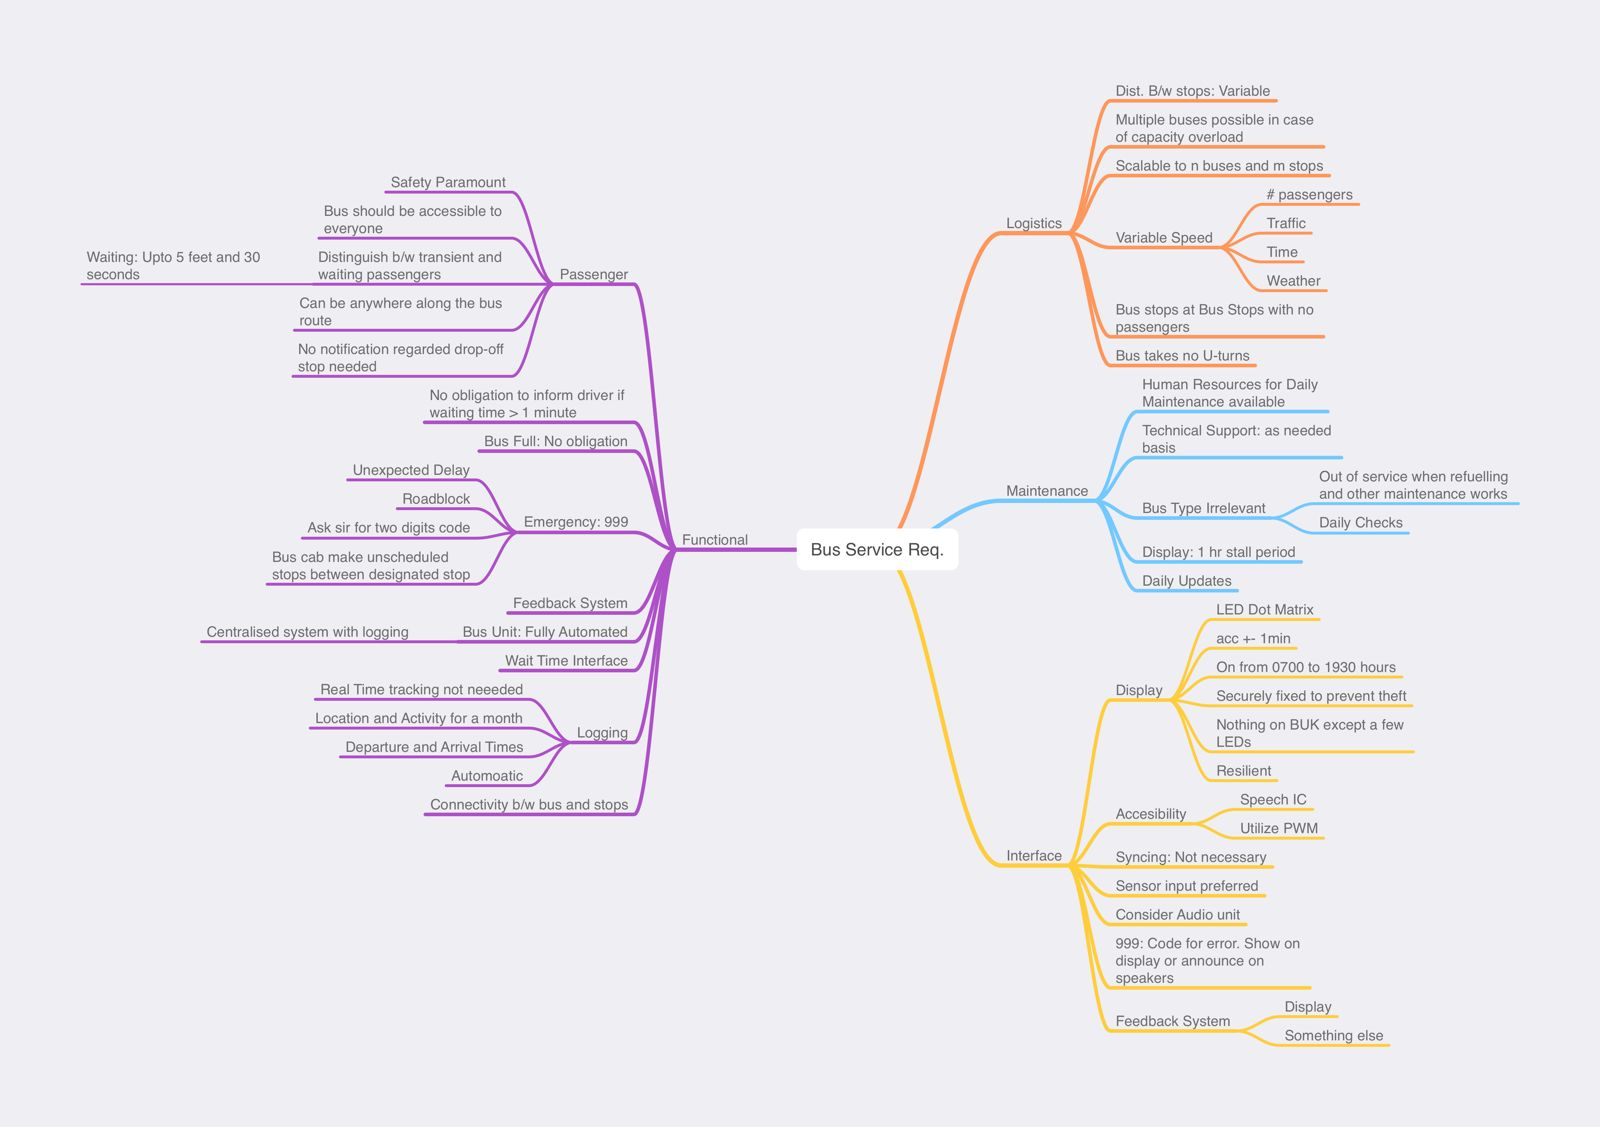
\includegraphics[width=0.9\textwidth,trim={1cm 0cm 0cm 2cm}, clip]{./Files/Images/MindMap.jpg}
        \caption{\textbf{Mind Map emphasizing the requirements} (Made using \textit{MindNote})}
    \end{figure}
    \end{center}
\newpage

\pagestyle{uselscape}
\savegeometry{before_landscape}
\begin{landscapes}
    \section{Project Management Details}

    
    \begin{figure}[H]
        \centering
        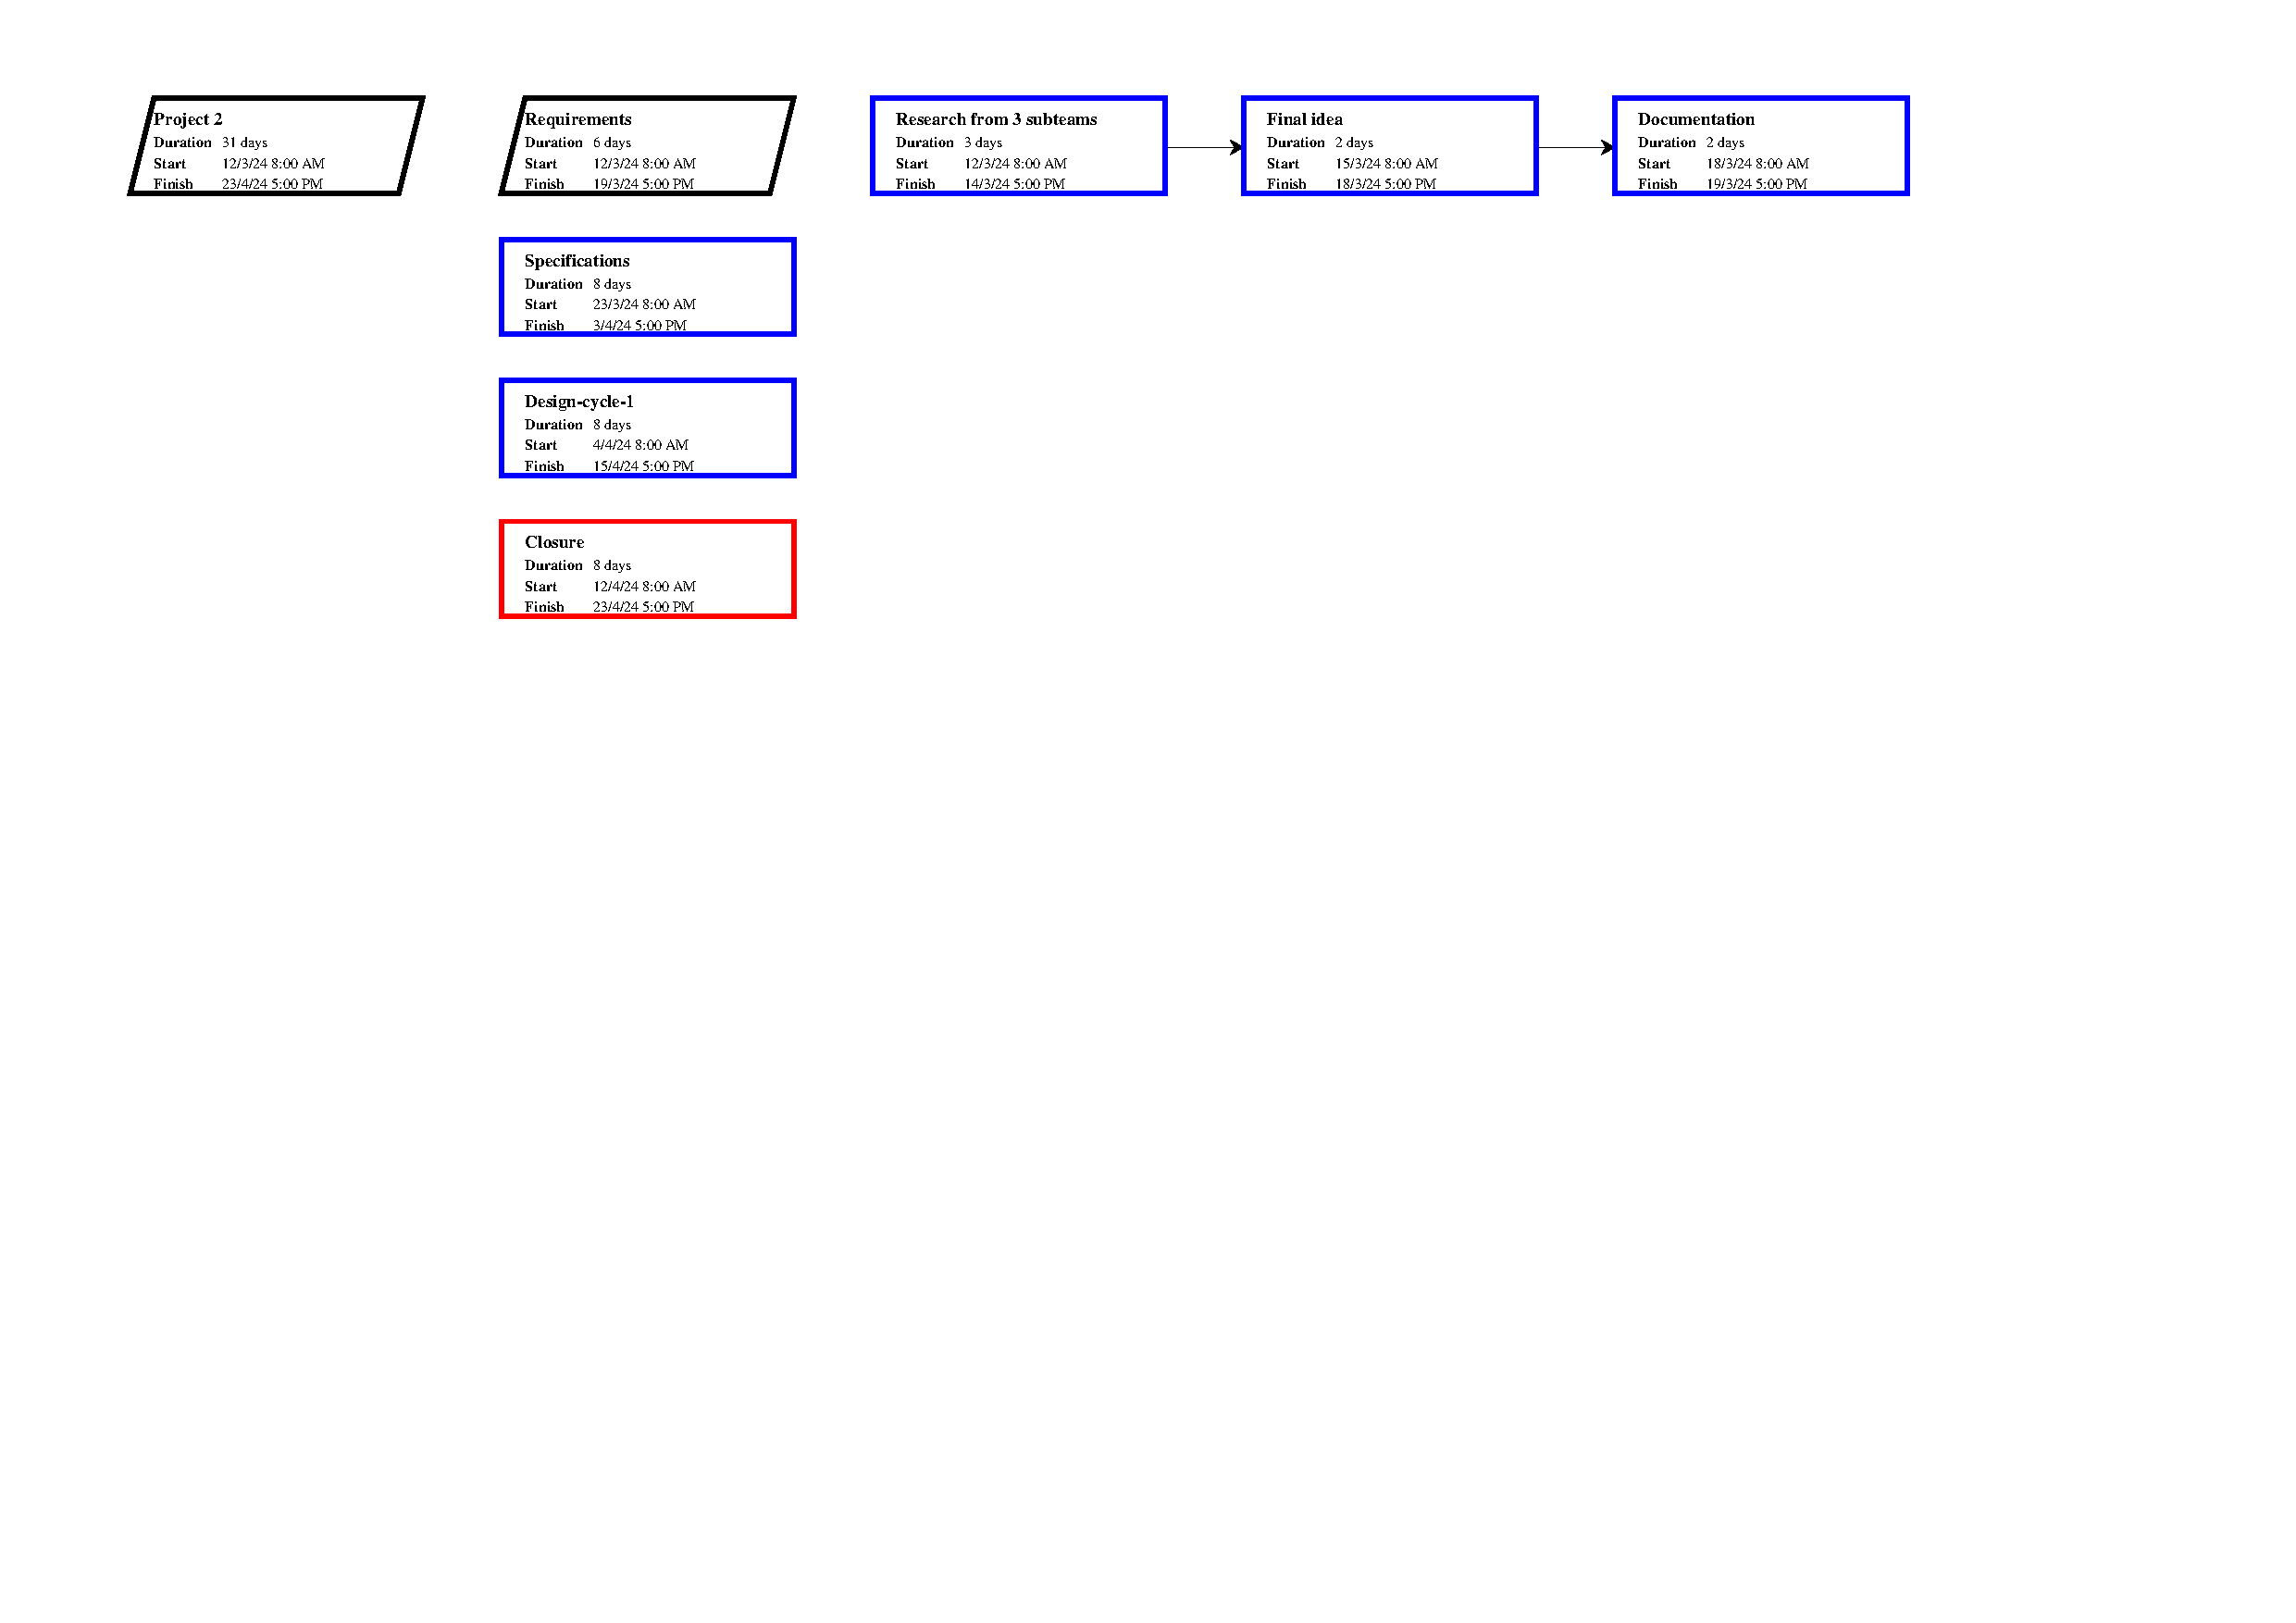
\includegraphics[width=1.1\textwidth, trim={0cm 14cm 0cm 0.5cm}, clip]{./Files/Images/Network.pdf}
        \caption[\textbf{Network Chart}]{\textbf{Network Chart} {(Created using \textit{Project Libre})}}
    \end{figure}
    %\footnotetext{Red boxes denote the critical path}
    
    \newpage
    
    \begin{figure}[H]
        \centering
        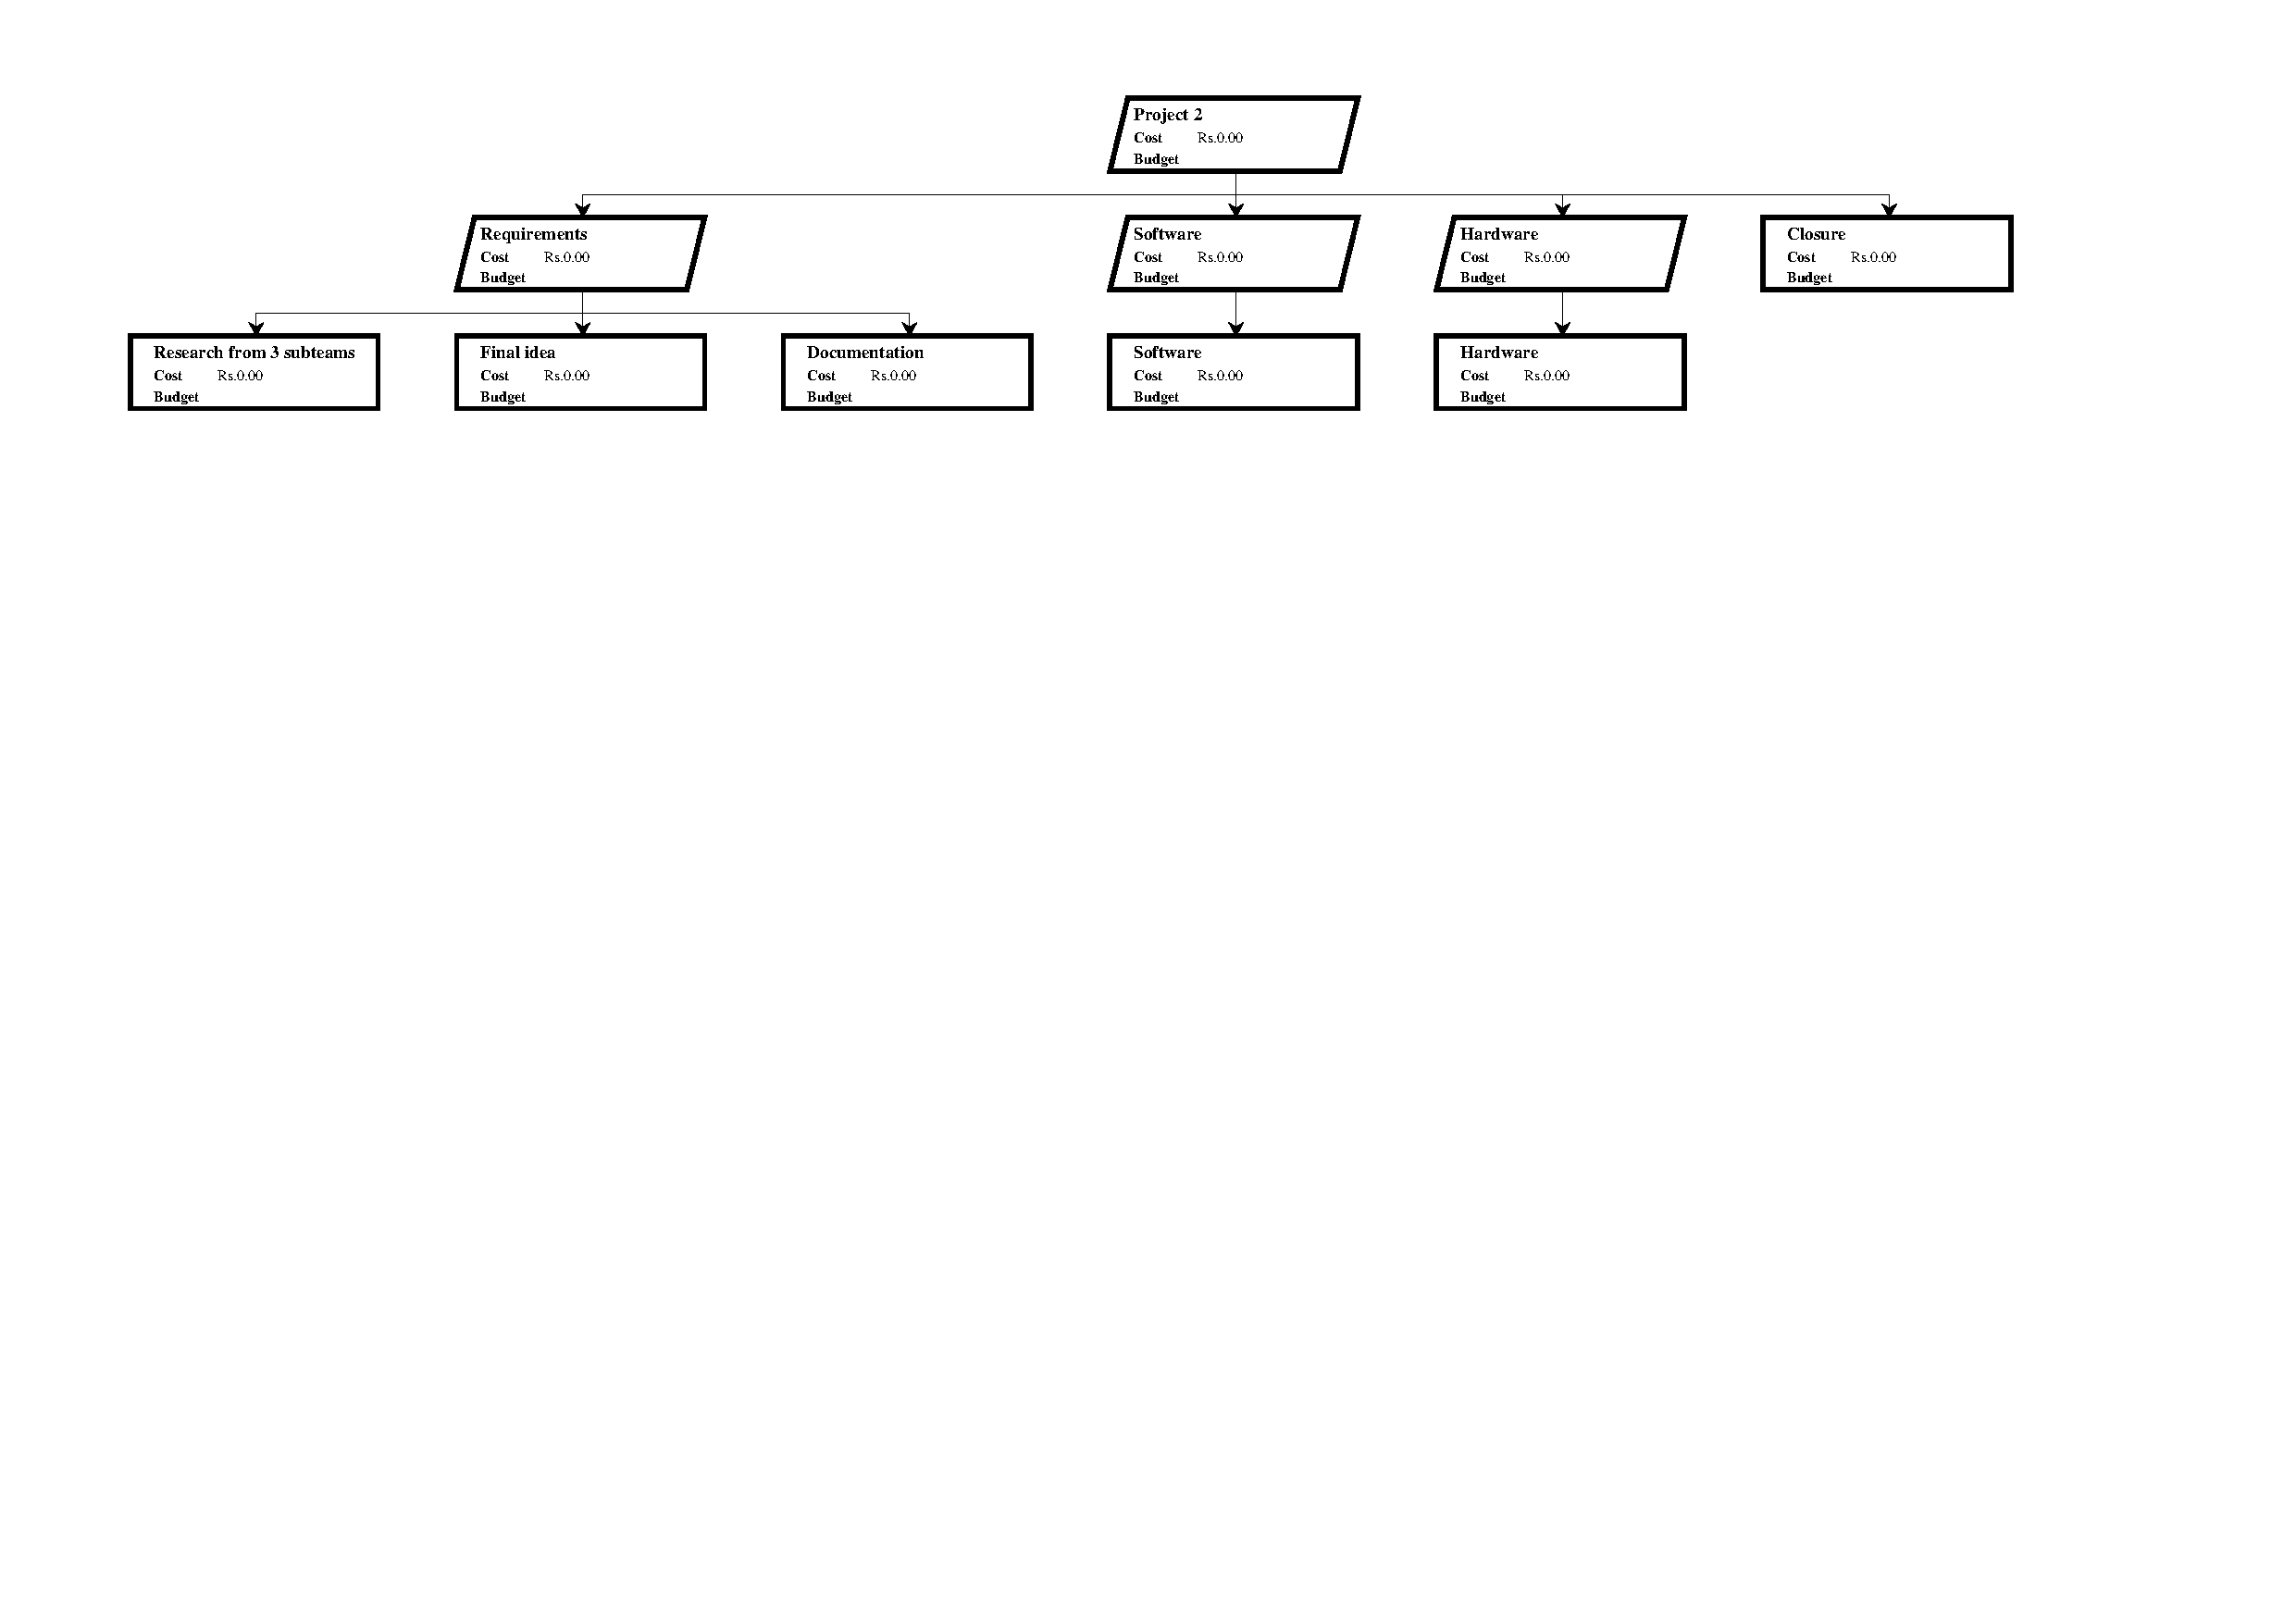
\includegraphics[width=1.1\textwidth, trim={0cm 14cm 0cm 0.5cm}, clip]{./Files/Images/WBS.pdf}
        \caption[\textbf{\ac{WBS} Chart}]{\textbf{\ac{WBS} Chart} {(Created using \textit{Project Libre})}}
    \end{figure}

    \newpage
    
    \begin{figure}[H]
        \centering
        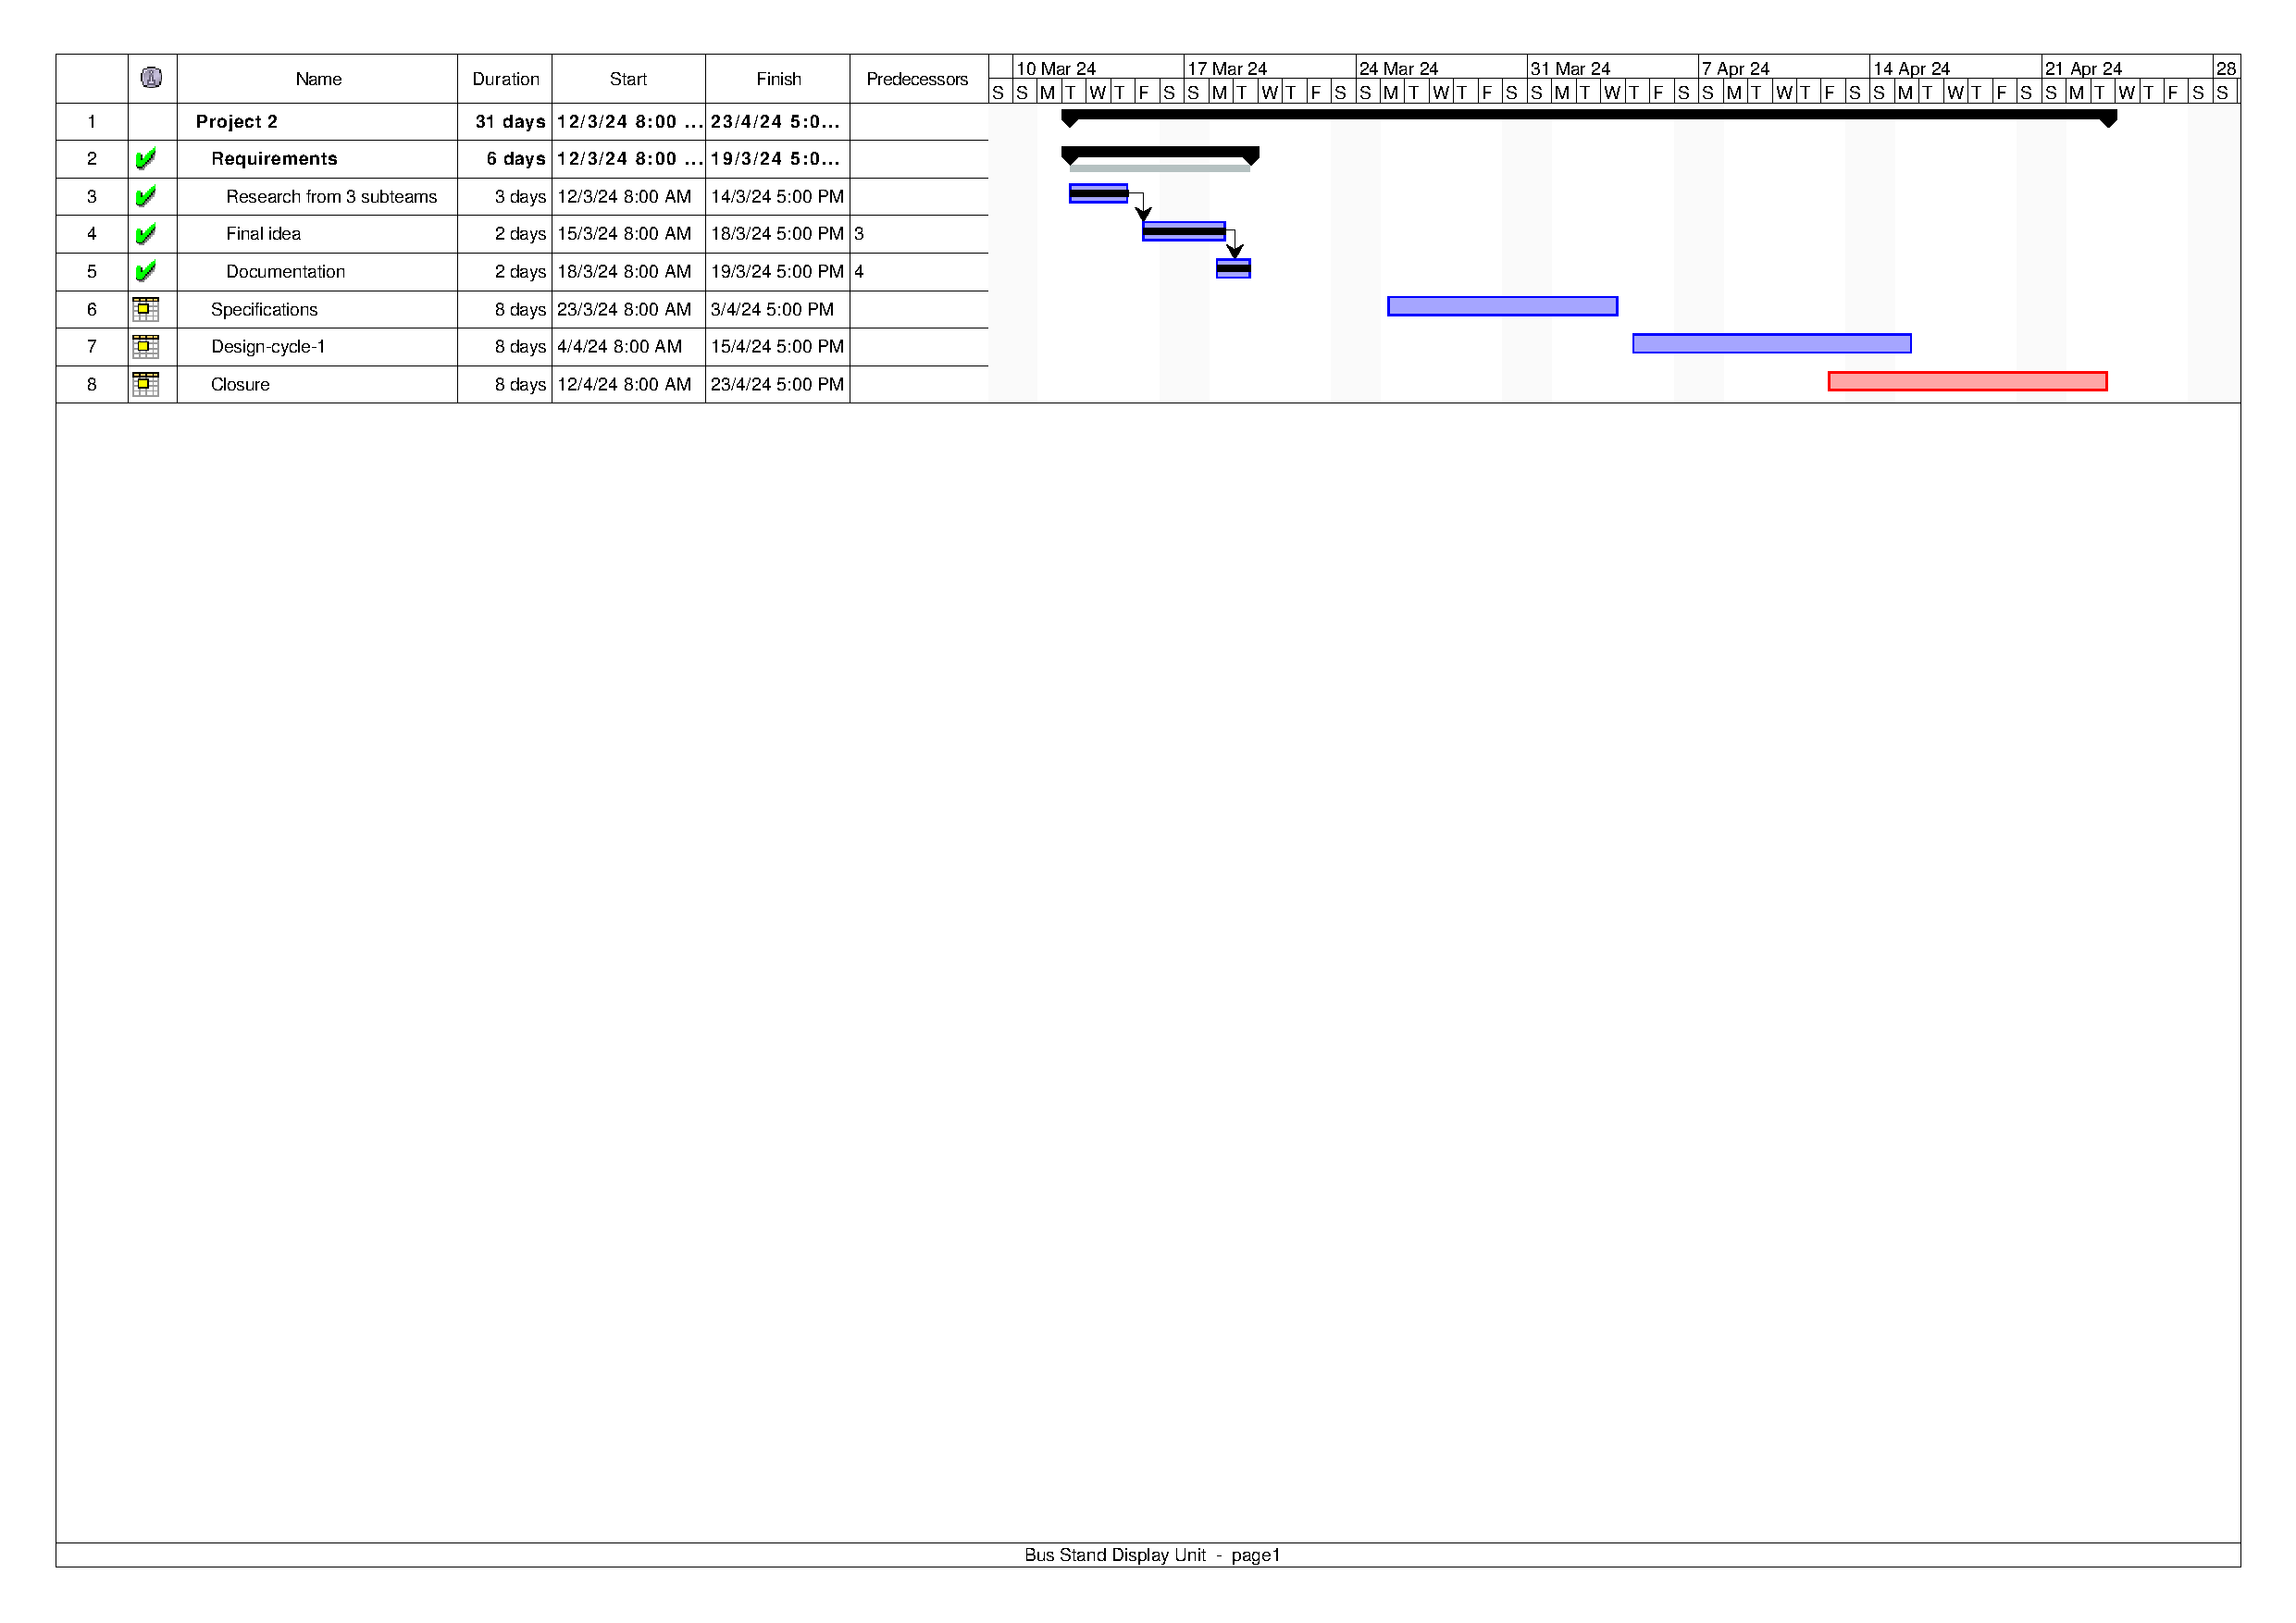
\includegraphics[width=1.1\textwidth, trim={0cm 22.3cm 0cm 0.5cm}, clip]{./Files/Images/Gantt.pdf}
        \caption[\textbf{Gantt Chart}]{\textbf{Gantt Chart} {(Created using \textit{Project Libre})}}
    \end{figure}

\end{landscapes}
\loadgeometry{before_landscape}

\begin{figure}[H]
	\begin{subfigure}[b]{\textwidth}
		\centering
		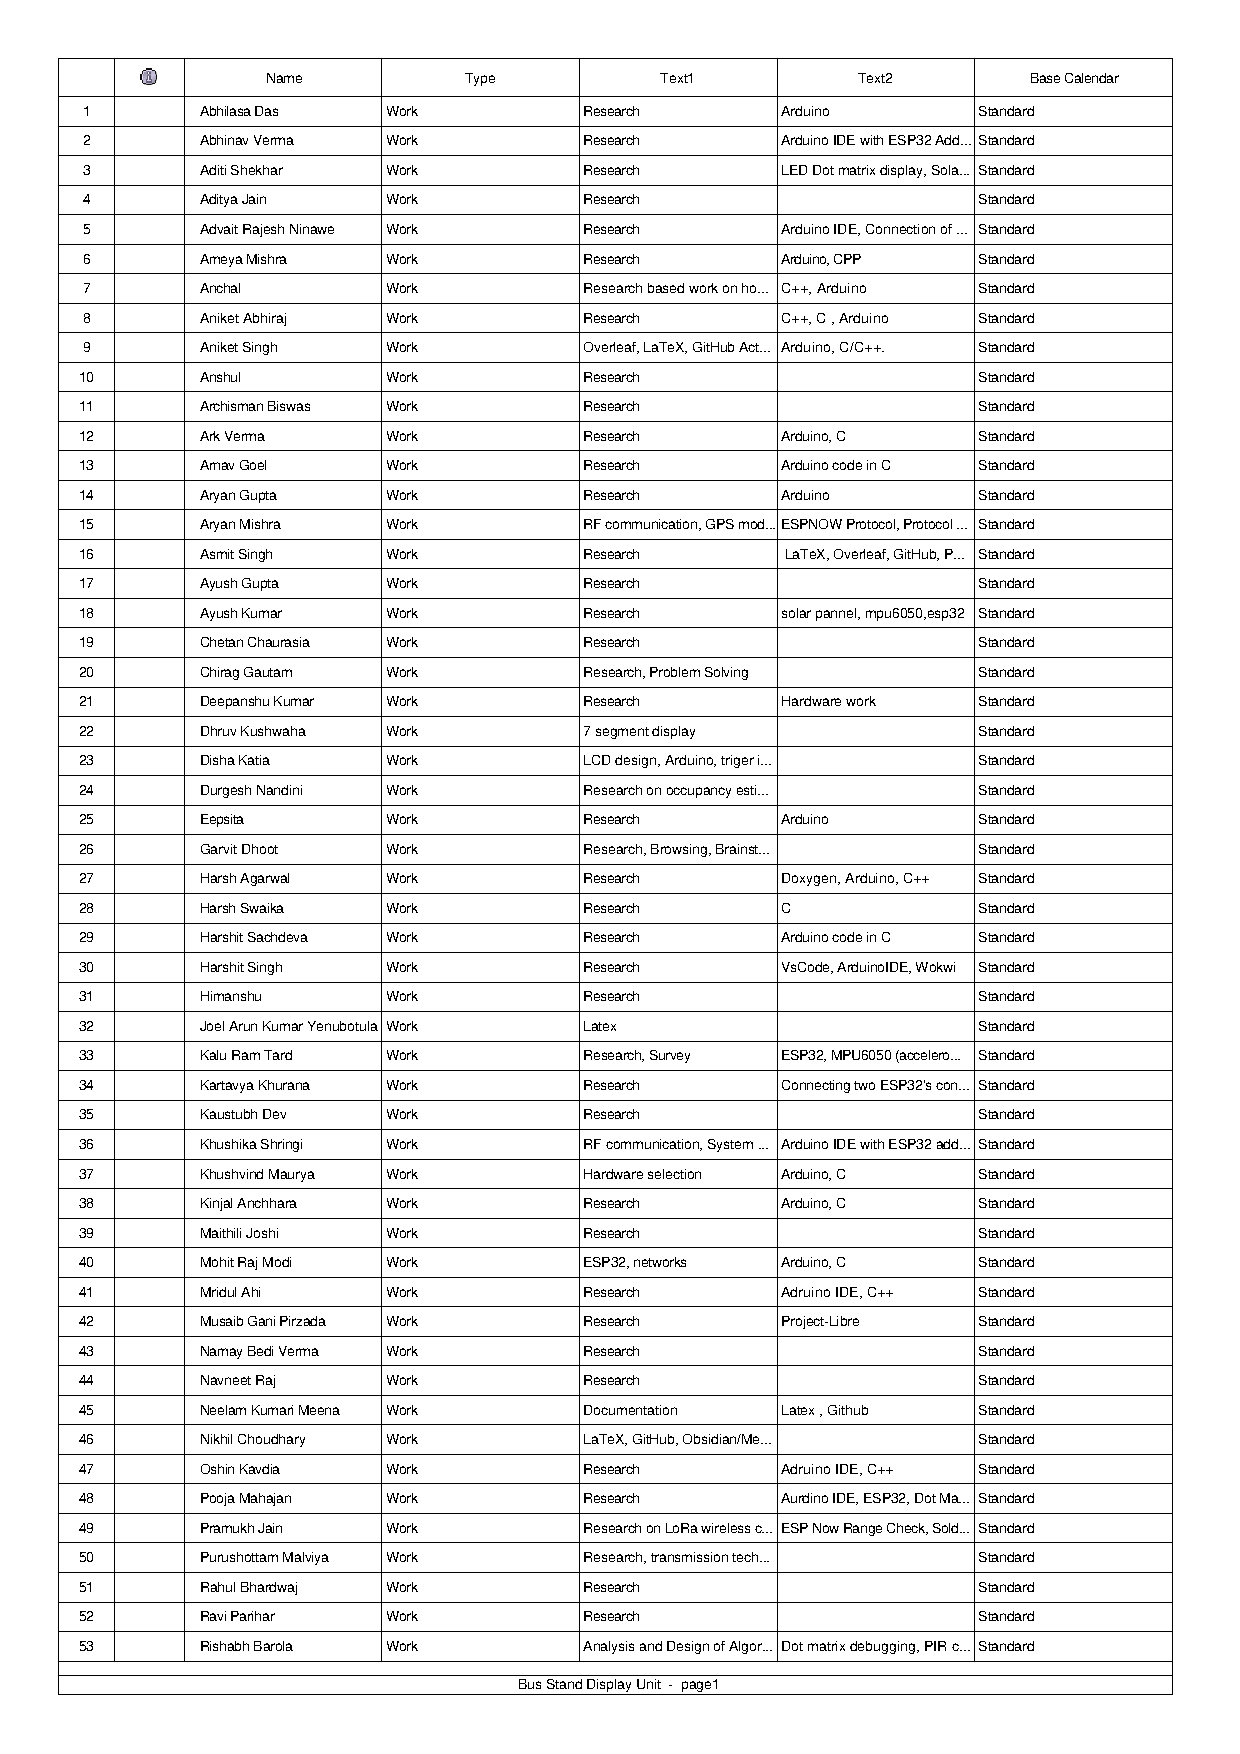
\includegraphics[page=1,width=\textwidth,trim={0cm 0cm 0cm 0cm}, clip]{./Files/Images/Resources.pdf}
		\caption{}
	\end{subfigure}
	\caption{\textbf{Resource Breakdown} {(Created using \textit{Project Libre})}}
\end{figure}

\newpage

\begin{figure}[H]
	\continuedfloat
	\begin{subfigure}[b]{\textwidth}
		\centering
		\includegraphics[page=2,width=\textwidth]{./Files/Images/Resources.pdf}
		\caption{}
	\end{subfigure}
	\caption{\textbf{Resource Breakdown} {(Created using \textit{Project Libre})}}
\end{figure}
\pagebreak

\pagenumbering{arabic}
\addcontentsline{toc}{section}{Abstract}
\begin{abstract}


\justify
This project introduces a system to assist users availing the bus facility inside the campus. Our solution consists of a Bus Mounted Unit that shows information about the bus's status on each bus as well as a sturdy, easily readable Display Unit at each stop that informs passengers of the bus's anticipated arrival time (as well as other important details). In addition to making an effort to be economical and energy-efficient, the system helps passengers by giving them important and beneficial details about the buses. This paper details the design process and technological integrations of this comprehensive bus assistance solution.

\end{abstract}



\section{Motivation}

The existing bus transit system on campus lacks effectiveness, accessibility, and convenience. Uncertain wait times make it challenging for passengers to decide whether to wait for the next bus or seek alternative transportation. Recognizing this limitation, we have developed a solution to address this issue and enhance the convenience of the bus transportation system for passengers. Our solution prioritizes sustainability by being energy-efficient and compliant with evolving regulations across various industries.



\pagebreak

%%%%%%%%%% Requirements %%%%%%%%%%%%%%%%


\chapter{Requirements}
\section{Functional Requirements}

\begin{enumerate}
    \item \underline{\textsc{Passenger Wait Times}} : Speeding to compensate for delays, even after a passenger waits over a minute and notifies the driver, is prohibited. Safety is paramount and arrival times may fluctuate accordingly.

    \item \underline{\textsc{Driver Notification}} : There's no obligation to inform the driver if a passenger waits for more than a minute. Waiting time is restricted to passenger boarding and deboarding.

    \item \underline{\textsc{Bus Full Indicator}} : The driver is not obligated to provide information to waiting passengers regarding the availability of space.

    \item \underline{\textsc{Road Incidents Update}} : When there's an unexpected delay or a roadblock, the display will flash '999' to signal an emergency.

    \item \index{Feedback Mechanism}\underline{\textsc{Feedback Mechanism}} : A digital interface could be implemented for users to provide feedback or report issues related to bus services.

    \item \index{Automation}\underline{\textsc{Automation of Bus Unit Operation}} :  It needs to be fully automated, manual input from the driver or staff for every bus direction change or stop is not expected.

    \item \underline{\textsc{Wait Time Interface}} : An interface can be devised to allow individuals heading to the bus stop to access information regarding the wait time.

    \item \underline{\textsc{Passenger Notification}} : Notifying the bus driver about a waiting passenger does not affect the bus route, even if the bus is empty.

    \item \underline{\textsc{Empty Bus Stops}} : The bus stops at empty bus stop as well, for passenger deboarding.

    \item \underline{\textsc{System Timeline}} : The desired timeline for the development, testing, and deployment of the system is April 25th, 2025.

    \item \index{Real-Time Tracking}\underline{\textsc{Real-Time Tracking}} : Real-time tracking of every bus is not required, but it is suggested to keep track of location and travel activity logs for around a month. Only have to keep a log of arrival and departure times at every bus stop, and this activity log is to be stored for the long term. (Can be done at appropriate frequency, no need for real time)

    \item \index{U-Turn}\underline{\textsc{Bus \gls{U-turn}}} : There may not be sufficient space at every stop for the bus to make a \gls{U-turn} and onboard passengers on the reverse path. Bus follows its route strictly, does not make U-Turns.

    \item \index{Accessibility}\underline{\textsc{Accessibility Priority}} : Prioritizing full accessibility for all campus residents on the bus service is not necessary.

    \item \underline{\textsc{Location Exchange}} : There's no need for each bus to be informed about the location of other buses.

    \item \underline{\textsc{Early Departure}} : Buses should not depart early, even if passengers have been waiting for over a minute, as it can confuse passengers and cause inconvenience.

    \item \underline{\textsc{Stop Wait Time}} : Buses typically aim to depart from each stop promptly after passengers have finished boarding and alighting.

    \item \underline{\textsc{Arrival and Departure Logging}} : The logging of bus arrival and departure must be automatic and cannot rely on manual input, ensuring accuracy and efficiency in tracking bus movements.

    \item \underline{\textsc{Centralized Management}} : The bus service is centrally managed, with everything logged. While there's no real-time monitoring, logs are available for review.

    \item \underline{\textsc{Passenger Drop-off Notification}} : There is no notification received when a passenger enters the bus regarding their drop-off.

    \item \underline{\textsc{Bus Bypass Protocol}} : If the bus is already full, the driver does not need to stop the bus at every subsequent stop.

    \item \underline{\textsc{Connectivity Focus}} :Connectivity is exclusively between buses and stops, with no direct communication link to passengers.

    \item \underline{\textsc{Capacity Information}} : It is unnecessary to display a bus's full status at upcoming stops, as passengers may alight at any point, which remains unpredictable to the driver.

    \item \underline{\textsc{Emergency Stops}} : In emergency situations, like a passenger feeling nauseous, the bus will make unscheduled stops between designated stops to address the issue and prioritizing passenger safety and well-being.

    \item \underline{\textsc{Waiting Passengers}} : The system should distinguish between transient presence and waiting passengers standing up to 5 feet from the bus stop pole for more than 30 seconds. Any passerby standing for 0.5 minutes would qualify them as a potential passenger, this wrong identification is allowed.

    \item \underline{\textsc{Following Route}} : Route to be followed and stops to be made should be a fully automated decision.

    \item \underline{\textsc{Location of Waiting Passengers}} : The passenger can be waiting anywhere along the route, not necessarily at the next bus stop.

    \item \underline{\textsc{Account for Delays}}: Assuming the bus may not always reach X at 8 AM sharp to start the shift.
\end{enumerate}

% \begin{enumerate}
%     \item \underline{\textsc{Passenger Wait Times and Safe Bus Speeds}} : Speeding to compensate for delays, even after a passenger waits over a minute and notifies the driver, is prohibited. Safety is paramount and arrival times may fluctuate accordingly.

%     \item \underline{\textsc{Updating Timings for Road Incidents}} : When there's an unexpected delay or a roadblock, the display will flash '999' to signal an emergency.

%     \item \underline{\textsc{Automation of Bus Operations}} :  It needs to be fully automated, manual input from the driver or staff for every bus direction change or stop is not expected.

%     \item \underline{\textsc{Bus Route and Passenger Notification}} : Notifying the bus driver about a waiting passenger does not affect the bus route, even if the bus is empty.

%     \item \underline{\textsc{Stopping at Empty Bus Stops}} : The bus is not expected to make stops at empty bus stops.

%     \item \underline{\textsc{Real-Time Bus Tracking}} : Real-time tracking of every bus is not required, but it is suggested to keep track of location and travel activity logs for around a month.

%     \item \underline{\textsc{Bus U-Turn for Passengers}} : There may not be sufficient space at every stop for the bus to make a U-turn and onboard passengers on the reverse path.

%     \item \underline{\textsc{Early Bus Departure}} : Buses should not depart early, even if passengers have been waiting for over a minute, as it can confuse passengers and cause inconvenience.

%     \item \underline{\textsc{Bus Stop Wait Time}} : Buses typically aim to depart from each stop promptly after passengers have finished boarding and alighting.

%     \item \underline{\textsc{Bus Arrival and Departure Logging}} : The logging of bus arrival and departure must be automatic and cannot rely on manual input, ensuring accuracy and efficiency in tracking bus movements.

%     \item \underline{\textsc{Centralized Bus Service Management}} : The bus service is centrally managed, with everything logged. While there's no real-time monitoring, logs are available for review.

%     \item \underline{\textsc{Passenger Drop-off Notification}} : There is no notification received when a passenger enters the bus regarding their drop-off.

%     \item \underline{\textsc{Bus Bypass Protocol}} : If the bus is already full, the driver does not need to stop the bus at every subsequent stop.

%     \item \underline{\textsc{Emergency Stops Policy}} : In emergency situations, like a passenger feeling nauseous, the bus will make unscheduled stops between designated stops to address the issue and prioritizing passenger safety and well-being.

%     \item \underline{\textsc{Differentiation of Waiting Passengers}} : The system should distinguish between transient presence and waiting passengers. Standing for 0.5 minutes qualifies someone as a potential passenger,with false positives accepted.
% \end{enumerate}

\section{Logistical Requirements}

\begin{enumerate}

\item \underline{\textsc{Stop Limits on Routes}} : The number of stops allowed between origin and destination is predetermined by the institute's system.

\item \underline{\textsc{Stop Distribution}} : The spacing between stops is not consistent and needs to be surveyed for accurate measurement.

\item \underline{\textsc{Simultaneous Bus Operation}} : If the number of passengers at the starting station exceeds the capacity of one bus, two buses can be operated simultaneously.

\item \underline{\textsc{Bus Deployment Adjustment}} : At the moment, there are only 2 buses available. The design needs to consider scalability aspects to accommodate demand fluctuations.

\item \underline{\textsc{Bus Speed Variability}} : Bus speed can vary depending on the amount of traffic, the number of passenger stops, the time of day, the weather, and the quality of the road.

\item \underline{\textsc{Availability of Alternative Transportation}} : No alternative transportation options are readily accessible to users.

\item \underline{\textsc{Scalability Considerations in Design Architecture}} : When designing the architecture, the primary scalability considerations to focus on are the number of buses and the number of stations.
\end{enumerate}
\section{Interface Requirements}

\begin{enumerate}
    \item \index{Display Method}\underline{\textsc{Display Method}} : Use of an \index{LED dot matrix display}\textit{\gls{LED dot matrix display}}{\tiny \textcolor{white}{\ac{LED}}}

    \item \underline{\textsc{Accuracy}} :The reading on the display must be accurate to ±1 minute

    \item \underline{\textsc{Duration Of Activity}} : Must remain active only between 0700 to 1930 hours, powering on/off should be automated

    \item \index{Display Mounting}\underline{\textsc{Display Mounting}} : Secure mounting to prevent theft. Mechanical fixation at unreachable height

    \item \underline{\textsc{Accessibility for Visually Impaired}} :  Utilize \ac{PWM} output or speech IC for accessibility

    \item \index{Syncing Capacity}\underline{\textsc{Syncing Capacity}} : Not necessary for synchronization

    \item \index{Budget Constraints}\underline{\textsc{Budget Constraints}} : To be Made as cost-efficient as possible

    \item \index{Passenger Input}\underline{\textsc{Passenger Input}} : Prefer sensor-based input

    \item \underline{\textsc{Audio Announcement}} : Consider installing an \textit{\gls{audio unit}}

    \item \index{BUk Functionality}\underline{\textsc{\ac{BUk} Functionality}} : No display on \ac{BUk}, includes some visual confirmation LEDs

    \item \underline{\textsc{Passenger Waiting Notification}} : Separate indicator integrated into BUk

    \item \index{Error Indicator}\underline{\textsc{Error Indicator}} : The Display would read ‘999’ to indicate emergency or unforeseen delays

    \item \underline{\textsc{Feedback System}} : Are there any means for taking feedback from the users or for reporting issues related to bus services?

    \item \underline{\textsc{Resilient}} : Display is exposed to all Delhi weather conditions

\end{enumerate}
\section{Readability Requirements}

\begin{enumerate}
    \item \index{Base Visibility}\underline{\textsc{Base Visibility}} : Must be readable from any point by a person with \index{6/6 vision}\textit{\gls{6/6 vision}} standing at upto 8 feet in front of the bus stop.

    \item \underline{\textsc{Visibility in Varied Weather}} : Clarification on visibility criteria under different weather conditions. Consideration of weather factors in New Delhi, including \textit{\gls{smog}} and rain.

    \item \underline{\textsc{Performance Metrics}} : Identification of specific performance metrics. Proposal to use start times, stop arrival/departure times, and out-of-service durations for evaluation.

\end{enumerate}
\section{Power Requirements}

\begin{enumerate}
    \item \index{Power Supply}\underline{\textsc{Power Supply}} : Display Unit must be battery-powered. Solar power to be used. It cannot be delivered directly to the \textit{\gls{embedded system}}

    \item \underline{\textsc{Alternative Power}} : Solar energy reliability in peak Delhi winter. Suggestions for backup power sources such as larger batteries or panels. Consensus needed on procurement across stakeholders

    \item \underline{\textsc{Connection Details}} : \\Solar Panel$\to$ AC/\ac{DC} converter $\to$ capacitor $\to$ \gls{embedded system} \\ \makebox[\linewidth]{OR}\\
          Solar Panel $\to$ \index{PWM converter}\gls{PWM converter} (or \index{MPPT converter}\gls{MPPT converter}) $\to$ \gls{USB} $\to$ \index{Embedded Systems}\Gls{embedded system}{\tiny \textcolor{white}{\ac{MPPT}}}

    \item \underline{\textsc{Location of Source of Solar Power}} :Must be installed at a nearby sunny point and directed to nearby bus stop
\end{enumerate}
\section{Maintenance Requirements}

\begin{enumerate}
    \item \underline{\textsc{Maintenance Feasibility}} : Human resources are available for daily maintenance of the stops, making monthly maintenance feasible.

    \item \index{Technical Support}\underline{\textsc{Technical Support}} : While the system is designed for minimal human intervention, technical support is available on an as-needed basis to address any technical issues that may arise.

    \item \underline{\textsc{Bus Maintenance}} : Bus type (electric or not) is not relevant .bus will be labeled as "Out of Service" during refueling, washing, and other maintenance issues. Maintenance checks to be carried out on a daily basis.

    \item \index{Display Malfunction}\underline{\textsc{Display Malfunction}} : In the event of an unforeseen malfunction in the display unit, a \textit{\gls{stall period}} of 1 hour will be allowed to fix the issue.

    \item \underline{\textsc{Daily Updates}} : Service is under the Transport Section which needs certain data to be provided on a daily basis.
\end{enumerate}



%%%%%%%%%% Specifications %%%%%%%%%%%%%%%%


\chapter{Specifications}
\section{\index{Backend Architecture}Backend Architecture Specifications}

\begin{itemize}
    \item There are $n$ buses: $0, 1, 2, \ldots n-1$
    \item There are $m$ stops: $0, 1, 2, \ldots m-1$  ($0$: first stop, $m-1$: last stop)
    \item We have to synchronize the \textit{\gls{24-hour clock}} at each stop
    \item In this system, all bus shifts end at the starting stop, i.e. the bus shift ends when the bus is back at the $0$\textsuperscript{th} stop. The sequence followed in a shift is \\
          {\bfseries $0$ $\to$ $1$ $\to$ $2$ $\to$ $3$ $\to$ \ldots $\to$ $m-2$ $\to$ $m-1$ $\to$ $m-2$ $\to$ \ldots$\to$ $3$ $\to$ $2$ $\to$ $1$ $\to$ $0$}\\
\end{itemize}

\begin{figure}[H]
        \centering
        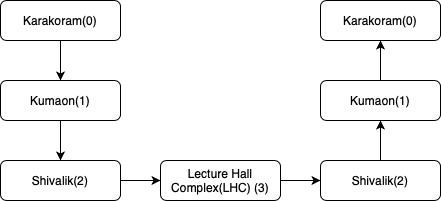
\includegraphics[width=0.7\textwidth]
        {./Files/Images/Flowchart.png}
        \caption{\textbf{Example for m = 4}} % Add a caption
    \end{figure}
    
\subsection{Data Storage and Timing Estimates}
\subsubsection{Over the Network}

\begin{enumerate}

\item Maintain the \textbf{Arrival}\textsubscript{mxn} matrix : Element $(i, j)$ stores the arrival time of $j$\textsuperscript{th} bus at the $i$\textsuperscript{th} stop
\item Maintain the \textbf{Departure}\textsubscript{mxn} matrix : Element $(i, j)$ stores the departure time of $j$\textsuperscript{th} bus at the $i$\textsuperscript{th} stop
\item Maintain the \textbf{PassengerWaitingAtStop}\textsubscript{1xm} matrix : Element $(0, j)$ is $x$ where
 \[ x = \begin{cases} \mbox{1} & \mbox{if any passenger is waiting at the j\textsuperscript{th} stop}  \\ \mbox{0} & \mbox{otherwise} \end{cases} \]
\item Maintain the \textbf{Direction}\textsubscript{1xn} matrix : Element (0, j) is x where
 \[ x = \begin{cases} \mbox{0} & \mbox{if $j$\textsuperscript{th} bus is moving towards $0$\textsuperscript{th} stop}  \\ \mbox{1} & \mbox{if $j$\textsuperscript{th} bus is moving towards $m-1$\textsuperscript{th} stop} \end{cases} \]


\end{enumerate}
\subsubsection{Locally}

\begin{itemize}

\item Maintain the \textbf{Scheduled}\textsubscript{mxn} matrix: Element (i, j) stores the scheduled time of the j\textsuperscript{th} bus at the i\textsuperscript{th} stop.
\item Maintain the \textbf{Estimated}\textsubscript{mxn} matrix: Element (i, j) stores the estimated time of the j\textsuperscript{th} bus at the i\textsuperscript{th} stop.
\item These matrices can be stored for estimation of arrival times, the passenger waiting functionality.
\item When j\textsuperscript{th} bus arrives at the i\textsuperscript{th} stop: (i, j)\textsuperscript{th} element of the \textbf{Arrival} matrix is updated. Bus stop `i' acts as the server, and all other bus stops act as clients.
\item When j\textsuperscript{th} bus departs the i\textsuperscript{th} stop: (i, j)\textsuperscript{th} element is updated. All arrival times of j\textsuperscript{th} column are updated to new estimate times based on \textit{average} time between stops and departure time from i\textsuperscript{th} stop.
\item For sensing whether the bus has stopped or not, we are using \textit{Accelerometer} reading.
\item \textbf{Bus stop nodes that can access this matrix} (i.e. nodes that are connected to the network):\\
\null \qquad Arrival time of next bus at i\textsuperscript{th} stop= min\{i\textsuperscript{th} row\}\\
\null \qquad Suppose that j the next bus arriving at i\textsuperscript{th} stop = j.\\
\null \qquad Direction of next bus = j\textsuperscript{th} element of \textbf{Direction} matrix.\\
\null \qquad Both Arrival time and Direction of buses needs to be communicated to the commuters.

\item \textbf{Bus stop nodes that cannot access this matrix} (i.e. nodes that unexpectedly get disconnected):\\
\null \qquad Arrival times of each bus estimated using scheduled time and last known whereabouts of buses:\\
\null \qquad \qquad Estimated time = Scheduled time + (last known deviation from scheduled\\
\null \qquad \qquad time)\\
\null \qquad If estimated time shows a large deviation from scheduled time, we will use scheduled time instead of estimated time.\\
\null \qquad Direction matrix can be updated based on these estimates: Direction of j\textsuperscript{th} bus switches when arrival time of stop m-1 is crossed.\\
\null \qquad Similar to the previous case, both Arrival time and Direction of buses needs to be communicated to the commuters.

\item \textbf{When the bus reaches stop 0 after a round trip}:\\
\null \qquad The \textbf{Arrival} and \textbf{Departure} matrices are updated to actual/estimated arrival and departure values, and this can be used to keep log of actual arrival and departure times in the system.\\
\null \qquad Moving average of previous runs can be used to refine predictions.\\
\null \qquad After uploading these times, we reset \textbf{Arrival} and \textbf{Departure} matrices to scheduled times.

\item \textbf{For more frequent time updates:}\\
\null \qquad We can specify some locations (using \textit{GPS}) where Wi-Fi is available on the route and send quick location updates to the network.\\
\null \qquad These locations can be used as \textit{pseudo-stops}, where the Bus Unit directly informs all Bus Stop nodes its location which can be further used to refine time predictions.
\end{itemize}
\subsection{Passenger waiting problem}

\begin{enumerate}

    \item We can use an \gls{ultrasonic sensor} at each stop to detect any passenger standing within 5 feet of the bus stop. If the sensor detects an obstacle within 5 feet for more than 30 seconds, then the (0, j)\textsuperscript{th} entry of \textbf{PassengerWaitingAtStop}\textsubscript{1xm} matrix is updated
    \item The bus unit stores a variable \textbf{PassengerWaiting} where\\
          \textbf{PassengerWaiting} = OR(all elements of \textbf{PassengerWaitingAtStop})
    \item This variable can be updated at every stop/pseudo stop

\end{enumerate}
\section{Frontend Specifications}
\subsection{Display Unit}
\begin{enumerate}
    \item These units will be mounted at every bus stop
    \item This unit will tell the time left for the buses from both direction to arrive at the station using the \textit{\gls{sliding text animation}}
    \item There will be one display unit per bus stop. Directional information will be displayed on the unit for buses from both directions
    \item When the units cannot connect to network, the time of arrival will be an extrapolation of the past arrival time data. The time of arrival will blink telling the maintenance staff that the unit is not connected to the network, but for the normal people it will be just the time of arrival
    \item The display unit will be \index{solar power}solar power. This is the connection to be followed: \\Solar Panel$\to$ AC/DC converter $\to$ capacitor $\to$ Embedded system \\ \makebox[\linewidth]{OR}\\
          Solar Panel $\to$ \index{PWM converter}\gls{PWM converter} (or \index{MPPT converter}\gls{MPPT converter}) $\to$ \ac{USB} $\to$ \index{Embedded Systems}Embedded Systems
\end{enumerate}
\subsection{Bus Mounted Units}
\begin{enumerate}
    \item Every bus will have a unit (BUk for the $k^{th}$ bus)
    \item The units will be powered from the battery of the bus
    \item While the bus is moving, these units will never be turned OFF
    \item These units will contain \textit{\gls{accelerometer}} (to determine the state of the bus whether it is moving or not)
    \item These units will also contain a RED switch, when pressed it will signal the system that the bus is OUT OF SERVICE
\end{enumerate}

\newpage
\section{Manpower Specifications}

\subsection{Man Hours}
\begin{center}
    \label{table:man_hours}
    \begin{longtable}{ | c | e | c | c| }
        \hline
        \multirow{2}{*}{\textbf{Name}} & \multirow{2}{*}{\textbf{Entry Number}} & \multirow{2}{*}{\textbf{Subtribe}} & \textbf{Man Hours} \\
                                       &                                        &                                    & \textbf{(in hrs)}  \\
        \hline \hline
        %%%
        Navneet Raj & 2021MT10240 & Documentation & 10.0\\ 
        \hline 
        Sanjay Pooniya & 2021EE10148 & Documentation & 3.0\\ 
        \hline 
        Ayush Gupta & 2021MT10697 & Documentation & 4.0\\ 
        \hline 
        Asmit Singh & 2021MT10887 & Documentation & 5.0\\ 
        \hline 
        Harsh Agarwal & 2021EE30977 & Research & 4.0\\ 
        \hline 
        Abhinav Verma & 2021EE10978 & Research & 10.0\\ 
        \hline 
        Khushika Shringi & 2021EE10665 & Research & 10.0\\ 
        \hline 
        Yash Goel & 2021EE10984 & Research & 9.0\\ 
        \hline 
        Aryan Gupta & 2021EE10974 & Research & 9.0\\ 
        \hline 
        Aniket Singh & 2021MT10256 & Research & 3.0\\ 
        \hline 
        2021ee10653 & 2021EE10653 & Research & 5.0\\ 
        \hline 
        Mridul Ahi & 2021MT10901 & Research & 1.0\\ 
        \hline 
        Eepsita & 2021EE10692 & Research & 7.0\\ 
        \hline 
        Pooja Mahajan & 2021EE10652 & Research & 9.0\\ 
        \hline 
        Chetan Chaurasia & 2021EE10147 & Research & 6.0\\ 
        \hline 
        Vikas Meena & 2021EE10169 & Research & 4.0\\ 
        \hline 
        Anshul & 2021EE10729 & Research & 5.0\\ 
        \hline 
        Ark Verma & 2021EE10783 & Research & 10.0\\ 
        \hline 
        Yash Agarwal & 2021EE10638 & Research & 8.0\\ 
        \hline 
        Sheetal Manatawal & 2021EE10174 & Research & 5.0\\ 
        \hline 
        Disha Katia & 2021EE10647 & Research & 6.5\\ 
        \hline 
        Chirag Gautam & 2021EE10166 & Research & 4.0\\ 
        \hline 
        Shubham Aggarwal & 2021EE10809 & Research & 8.0\\ 
        \hline 
        Mohit Raj & 2021MT10919 & Research & 5.0\\ 
        \hline 
        Ujjwal Yadav & 2021EE10669 & Research & 8.0\\ 
        \hline 
        Aniket Abhiraj & 2021EE10676 & Research & 9.0\\ 
        \hline 
        Sarthak Kumar Singh & 2021EE10673 & Research & 8.0\\ 
        \hline 
        Aditi Shekhar & 2021EE10685 & Research & 6.0\\ 
        \hline 
        Anchal & 2021MT10910 & Research & 8.0\\ 
        \hline 
        Rohan Das & 2021EE10621 & Research & 7.0\\ 
        \hline 
        Rohan Das & 2021EE10621 & Research & 7.0\\ 
        \hline 
        Harsh Swaika & 2021EE11052 & Research & 4.0\\ 
        \hline 
        Aditya Jain & 2021EE10633 & Research & 7.0\\ 
        \hline 
        Harshit Sachdeva & 2021EE30705 & Research & 7.0\\ 
        \hline 
        Kinjal Anchhara & 2021MT60959 & Research & 8.0\\ 
        \hline 
        Dhruv Kushwaha & 2021MT10235 & Research & 6.0\\ 
        \hline 
        Shubh Chhabra & 2021EE10645 & Research & 8.0\\ 
        \hline 
        Rishabh Barola & 2021EE10636 & Research & 5.0\\ 
        \hline 
        Pramukh Jain & 2021EE10720 & Research & 6.0\\ 
        \hline 
        Oshin Kavdia & 2021EE10654 & Research & 4.0\\ 
        \hline 
        Kalu Ram Tard & 2021EE10680 & Research & 8.0\\ 
        \hline 
        Joel Arun Kumar Yenubotula & 2021EE10159 & Research & 5.0\\ 
        \hline 
        Ameya Mishra & 2021MT10637 & Research & 9.0\\ 
        \hline 
        Tanmai Merugu & 2021EE10149 & Research & 8.0\\ 
        \hline 
        Khushvind Maurya & 2021MT10238 & Research & 3.5\\ 
        \hline 
        Vinay Sah & 2021EE10171 & Research & 3.0\\ 
        \hline 
        Vasu Sharma & 2021EE10620 & Research & 9.0\\ 
        \hline 
        Shivam Kumar & 2021EE10165 & Research & 4.0\\ 
        \hline 
        Deepanshu Kumar & 2021EE10696 & Research & 4.0\\ 
        \hline 
        Durgesh Nandini & 2021EE10651 & Research & 8.0\\ 
        \hline 
        Kaustubh Dev & 2021EE10689 & Research & 8.0\\ 
        \hline 
        Arnav Goel & 2021EE10699 & Research & 7.0\\ 
        \hline 
        Ayush Kumar & 2021EE10150 & Research & 5.0\\ 
        \hline 
        Bingi Sai Vishal & 2021EE10668 & Research & 6.0\\ 
        \hline 
        Abhilasa Das & 2021EE10168 & Research & 8.0\\ 
        \hline 
        Ravi Parihar & 2021EE10156 & Research & 4.0\\ 
        \hline 
        Himanshu Prajapati & 2021EE30177 & Research & 4.0\\ 
        \hline 
        Aryan Mishra & 2021EE10137 & Research & 10.0\\ 
        \hline 

        %%%
        \hline
        \caption{Manpower Specifications}
    \end{longtable}
\end{center}

\newpage
\subsection{Skillsets Acquired}
\begin{center}
    \label{table:skillsets}
    \begin{longtable}{ | c | c | m{6cm} | }
        \hline
        \textbf{Name}              & \textbf{Subtribe} & \textbf{Skillsets Acquired}                                             \\
        \hline \hline
        %%%
        Navneet Raj & Documentation & Overleaf, LaTeX, GitHub Actions, Pandoc\\ 
        \hline 
        Sanjay Pooniya & Documentation & Latex\\ 
        \hline 
        Ayush Gupta & Documentation & Research\\ 
        \hline 
        Asmit Singh & Documentation & Documentation\\ 
        \hline 
        Harsh Agarwal & Research & Research\\ 
        \hline 
        Abhinav Verma & Research & Research\\ 
        \hline 
        Khushika Shringi & Research & Research\\ 
        \hline 
        Yash Goel & Research & Research\\ 
        \hline 
        Aryan Gupta & Research & Research\\ 
        \hline 
        Aniket Singh & Research & Data transfer with minimum internet usage\\ 
        \hline 
        2021ee10653 & Research & Research\\ 
        \hline 
        Mridul Ahi & Research & Research\\ 
        \hline 
        Eepsita & Research & Research\\ 
        \hline 
        Pooja Mahajan & Research & Research\\ 
        \hline 
        Chetan Chaurasia & Research & Research\\ 
        \hline 
        Vikas Meena & Research & Research\\ 
        \hline 
        Anshul & Research & Research\\ 
        \hline 
        Ark Verma & Research & RF communication, GPS modules, Telemetry, Research\\ 
        \hline 
        Yash Agarwal & Research & Research\\ 
        \hline 
        Sheetal Manatawal & Research & Research\\ 
        \hline 
        Disha Katia & Research & Research\\ 
        \hline 
        Chirag Gautam & Research & Research\\ 
        \hline 
        Shubham Aggarwal & Research & Research, Problem Solving\\ 
        \hline 
        Mohit Raj & Research & Research\\ 
        \hline 
        Ujjwal Yadav & Research & 7 Segment Display\\ 
        \hline 
        Aniket Abhiraj & Research & LCD design, Arduino, Trigger identifier for bus, Hardware design.\\ 
        \hline 
        Sarthak Kumar Singh & Research & Research on occupancy estimation\\ 
        \hline 
        Aditi Shekhar & Research & Research\\ 
        \hline 
        Anchal & Research & Research, Browsing, Brainstorming\\ 
        \hline 
        Rohan Das & Research & Research\\ 
        \hline 
        Rohan Das & Research & Research\\ 
        \hline 
        Harsh Swaika & Research & Research\\ 
        \hline 
        Aditya Jain & Research & Research\\ 
        \hline 
        Harshit Sachdeva & Research & Research\\ 
        \hline 
        Kinjal Anchhara & Research & Research\\ 
        \hline 
        Dhruv Kushwaha & Research & Research, Survey\\ 
        \hline 
        Shubh Chhabra & Research & Research\\ 
        \hline 
        Rishabh Barola & Research & RF communication, System design\\ 
        \hline 
        Pramukh Jain & Research & Hardware selection\\ 
        \hline 
        Oshin Kavdia & Research & Research\\ 
        \hline 
        Kalu Ram Tard & Research & Research\\ 
        \hline 
        Joel Arun Kumar Yenubotula & Research & ESP32, Networks\\ 
        \hline 
        Ameya Mishra & Research & Research\\ 
        \hline 
        Tanmai Merugu & Research & Research\\ 
        \hline 
        Khushvind Maurya & Research & Research\\ 
        \hline 
        Vinay Sah & Research & Research\\ 
        \hline 
        Vasu Sharma & Research & LaTeX, GitHub, Obsidian/Mermaid, MSWord\\ 
        \hline 
        Shivam Kumar & Research & Research\\ 
        \hline 
        Deepanshu Kumar & Research & Research\\ 
        \hline 
        Durgesh Nandini & Research & Research on LoRa wireless comminication\\ 
        \hline 
        Kaustubh Dev & Research & Research, Transmission techniques, Receiver hardware\\ 
        \hline 
        Arnav Goel & Research & Research\\ 
        \hline 
        Ayush Kumar & Research & Research\\ 
        \hline 
        Bingi Sai Vishal & Research & Analysis and Design of Algorithms, python\\ 
        \hline 
        Abhilasa Das & Research & Research\\ 
        \hline 
        Ravi Parihar & Research & Research\\ 
        \hline 
        Himanshu Prajapati & Research & GitHub, Research on YT\\ 
        \hline 
        Aryan Mishra & Research & Research\\ 
        \hline 

        %%%
        \hline
        \caption{Skillsets Acquired}
    \end{longtable}
\end{center}

\newpage
\subsection{Competency Matrix}
\begin{center}
\label{table:competency}
\setlength\LTleft{-1.4cm}
\begin{longtable}{|c|c|c|c|c|c|p{1.2cm}|c|c|} \hline
Name                    & Python                   & LaTeX                    & Excel                    & GitHub                   & Pandoc                   & Project Libre            & Obsidian                 & Zotero                   \\ \hline
Saket Kandoi            & \cellcolor[HTML]{00B050} & \cellcolor[HTML]{92D050} & \cellcolor[HTML]{00B050} & \cellcolor[HTML]{00B050} & \cellcolor[HTML]{FFC000} & \cellcolor[HTML]{D9D9D9} & \cellcolor[HTML]{00B050} & \cellcolor[HTML]{FFC000} \\ \hline
Dintyala Rahul Bhardwaj & \cellcolor[HTML]{FFFF00} & \cellcolor[HTML]{00B050} & \cellcolor[HTML]{00B050} & \cellcolor[HTML]{FFFF00} & \cellcolor[HTML]{FFC000} & \cellcolor[HTML]{FFC000} & \cellcolor[HTML]{00B050} & \cellcolor[HTML]{FFC000} \\ \hline
Archisman Biswas        & \cellcolor[HTML]{00B050} & \cellcolor[HTML]{92D050} & \cellcolor[HTML]{92D050} & \cellcolor[HTML]{00B050} & \cellcolor[HTML]{FFFF00} & \cellcolor[HTML]{D9D9D9} & \cellcolor[HTML]{FFC000} & \cellcolor[HTML]{FFC000} \\ \hline
Sanjay Pooniya          & \cellcolor[HTML]{FFFF00} & \cellcolor[HTML]{92D050} & \cellcolor[HTML]{FFFF00} & \cellcolor[HTML]{92D050} & \cellcolor[HTML]{FFC000} & \cellcolor[HTML]{FFC000} & \cellcolor[HTML]{FFC000} & \cellcolor[HTML]{D9D9D9} \\ \hline
Nikhil Choudhary        & \cellcolor[HTML]{FFFF00} & \cellcolor[HTML]{92D050} & \cellcolor[HTML]{FFFF00} & \cellcolor[HTML]{FFFF00} & \cellcolor[HTML]{D9D9D9} & \cellcolor[HTML]{FFFF00} & \cellcolor[HTML]{FFC000} & \cellcolor[HTML]{00B050} \\ \hline
Navneet Raj             & \cellcolor[HTML]{00B050} & \cellcolor[HTML]{FFFF00} & \cellcolor[HTML]{FFFF00} & \cellcolor[HTML]{00B050} & \cellcolor[HTML]{FFFF00} & \cellcolor[HTML]{D9D9D9} & \cellcolor[HTML]{92D050} & \cellcolor[HTML]{D9D9D9} \\ \hline
Aryan Mishra            & \cellcolor[HTML]{92D050} & \cellcolor[HTML]{00B050} & \cellcolor[HTML]{92D050} & \cellcolor[HTML]{FFFF00} & \cellcolor[HTML]{FFFF00} & \cellcolor[HTML]{FFFF00} & \cellcolor[HTML]{00B050} & \cellcolor[HTML]{FFFF00} \\ \hline
Purushottam Malviya     & \cellcolor[HTML]{FFFF00} & \cellcolor[HTML]{FFFF00} & \cellcolor[HTML]{FFFF00} & \cellcolor[HTML]{FFC000} & \cellcolor[HTML]{D9D9D9} & \cellcolor[HTML]{D9D9D9} & \cellcolor[HTML]{D9D9D9} & \cellcolor[HTML]{FFC000} \\ \hline
Musaib Gani Pirzada     & \cellcolor[HTML]{00B050} & \cellcolor[HTML]{FFFF00} & \cellcolor[HTML]{FFFF00} & \cellcolor[HTML]{92D050} & \cellcolor[HTML]{FFFF00} & \cellcolor[HTML]{00B050} & \cellcolor[HTML]{FFC000} & \cellcolor[HTML]{FFC000} \\ \hline
Vaibhav Seth            & \cellcolor[HTML]{00B050} & \cellcolor[HTML]{92D050} & \cellcolor[HTML]{FFFF00} & \cellcolor[HTML]{92D050} & \cellcolor[HTML]{D9D9D9} & \cellcolor[HTML]{D9D9D9} & \cellcolor[HTML]{FFC000} & \cellcolor[HTML]{D9D9D9} \\ \hline
Sanskriti Gautam        & \cellcolor[HTML]{FFFF00} & \cellcolor[HTML]{92D050} & \cellcolor[HTML]{FFFF00} & \cellcolor[HTML]{FFFF00} & \cellcolor[HTML]{FFC000} & \cellcolor[HTML]{FFC000} & \cellcolor[HTML]{D9D9D9} & \cellcolor[HTML]{D9D9D9} \\ \hline
Asmit Singh             & \cellcolor[HTML]{92D050} & \cellcolor[HTML]{FFFF00} & \cellcolor[HTML]{00B050} & \cellcolor[HTML]{FFFF00} & \cellcolor[HTML]{D9D9D9} & \cellcolor[HTML]{D9D9D9} & \cellcolor[HTML]{D9D9D9} & \cellcolor[HTML]{D9D9D9} \\ \hline
\caption{Competency Matrix for Documentation Team}
\end{longtable}
\setlength\LTleft{0cm}
\end{center}


\begin{center}
\label{table:competency_apd}
\begin{longtable}{|c|c|c|c|c|c|p{1.2cm}|c|c|}
\hline
Name                & Arduino                  & C                        & Doxygen                  & Wokwi                    \\ \hline
Shubham Aggarwal    & \cellcolor[HTML]{92D050} & \cellcolor[HTML]{00B050} & \cellcolor[HTML]{FFC000} & \cellcolor[HTML]{FFFF00} \\ \hline
Mridul Ahi          & \cellcolor[HTML]{92D050} & \cellcolor[HTML]{00B050} & \cellcolor[HTML]{F2F2F2} & \cellcolor[HTML]{F2F2F2} \\ \hline
Abhinav Verma       & \cellcolor[HTML]{92D050} & \cellcolor[HTML]{00B050} & \cellcolor[HTML]{FFC000} & \cellcolor[HTML]{FFC000} \\ \hline
Aryan Gupta         & \cellcolor[HTML]{FFFF00} & \cellcolor[HTML]{FFFF00} & \cellcolor[HTML]{F2F2F2} & \cellcolor[HTML]{F2F2F2} \\ \hline
Khushika Shringi    & \cellcolor[HTML]{92D050} & \cellcolor[HTML]{92D050} & \cellcolor[HTML]{F2F2F2} & \cellcolor[HTML]{FFC000} \\ \hline
Vasu Sharma         & \cellcolor[HTML]{FFFF00} & \cellcolor[HTML]{00B050} & \cellcolor[HTML]{F2F2F2} & \cellcolor[HTML]{FFC000} \\ \hline
Ark Verma           & \cellcolor[HTML]{FFFF00} & \cellcolor[HTML]{00B050} & \cellcolor[HTML]{F2F2F2} & \cellcolor[HTML]{F2F2F2} \\ \hline
Oshin Kavdia        & \cellcolor[HTML]{FFFF00} & \cellcolor[HTML]{00B050} & \cellcolor[HTML]{F2F2F2} & \cellcolor[HTML]{F2F2F2} \\ \hline
Sarthak Kumar Singh & \cellcolor[HTML]{FFFF00} & \cellcolor[HTML]{00B050} & \cellcolor[HTML]{F2F2F2} & \cellcolor[HTML]{F2F2F2} \\ \hline
Harsh Agarwal       & \cellcolor[HTML]{92D050} & \cellcolor[HTML]{92D050} & \cellcolor[HTML]{FFC000} & \cellcolor[HTML]{F2F2F2} \\ \hline
Aditya Jain       & \cellcolor[HTML]{92D050} & \cellcolor[HTML]{92D050} & \cellcolor[HTML]{FFC000} & \cellcolor[HTML]{FFFF00} \\ \hline
Anchal       & \cellcolor[HTML]{92D050} & \cellcolor[HTML]{92D050} & \cellcolor[HTML]{FFFF00} & \cellcolor[HTML]{FFFF00} \\ \hline
Ameya Mishra      & \cellcolor[HTML]{FFFF00} & \cellcolor[HTML]{92D050} & \cellcolor[HTML]{F2F2F2} & \cellcolor[HTML]{F2F2F2} \\ \hline
Aniket Abhiraj    & \cellcolor[HTML]{92D050} & \cellcolor[HTML]{92D050} & \cellcolor[HTML]{F2F2F2} & \cellcolor[HTML]{F2F2F2} \\ \hline
Aniket Singh      & \cellcolor[HTML]{92D050} & \cellcolor[HTML]{00B050} & \cellcolor[HTML]{F2F2F2} & \cellcolor[HTML]{FFC000} \\ \hline
Anshul            & \cellcolor[HTML]{FFFF00} & \cellcolor[HTML]{FFFF00} & \cellcolor[HTML]{F2F2F2} & \cellcolor[HTML]{FFC000} \\ \hline
Arnav Goel        & \cellcolor[HTML]{92D050} & \cellcolor[HTML]{92D050} & \cellcolor[HTML]{F2F2F2} & \cellcolor[HTML]{FFC000} \\ \hline
Dhruv Kushwaha    & \cellcolor[HTML]{92D050} & \cellcolor[HTML]{00B050} & \cellcolor[HTML]{F2F2F2} & \cellcolor[HTML]{F2F2F2} \\ \hline
Harsh Swaika      & \cellcolor[HTML]{92D050} & \cellcolor[HTML]{92D050} & \cellcolor[HTML]{FFC000} & \cellcolor[HTML]{F2F2F2} \\ \hline
Harshit Sachdeva  & \cellcolor[HTML]{92D050} & \cellcolor[HTML]{FFFF00} & \cellcolor[HTML]{F2F2F2} & \cellcolor[HTML]{F2F2F2} \\ \hline
Harshit Singh     & \cellcolor[HTML]{92D050} & \cellcolor[HTML]{00B050} & \cellcolor[HTML]{FFC000} & \cellcolor[HTML]{F2F2F2} \\ \hline
Kaustubh Dev      & \cellcolor[HTML]{FFFF00} & \cellcolor[HTML]{92D050} & \cellcolor[HTML]{FFC000} & \cellcolor[HTML]{F2F2F2} \\ \hline
Khushvind Maurya  & \cellcolor[HTML]{92D050} & \cellcolor[HTML]{92D050} & \cellcolor[HTML]{F2F2F2} & \cellcolor[HTML]{F2F2F2} \\ \hline
Kinjal Anchhara   & \cellcolor[HTML]{92D050} & \cellcolor[HTML]{00B050} & \cellcolor[HTML]{F2F2F2} & \cellcolor[HTML]{F2F2F2} \\ \hline
Maithili Joshi    & \cellcolor[HTML]{92D050} & \cellcolor[HTML]{00B050} & \cellcolor[HTML]{F2F2F2} & \cellcolor[HTML]{F2F2F2} \\ \hline
Mohit Raj Modi    & \cellcolor[HTML]{92D050} & \cellcolor[HTML]{92D050} & \cellcolor[HTML]{F2F2F2} & \cellcolor[HTML]{F2F2F2} \\ \hline
Mridul Ahi        & \cellcolor[HTML]{FFFF00} & \cellcolor[HTML]{92D050} & \cellcolor[HTML]{FFC000} & \cellcolor[HTML]{F2F2F2} \\ \hline
Namay Bedi Verma  & \cellcolor[HTML]{92D050} & \cellcolor[HTML]{92D050} & \cellcolor[HTML]{FFC000} & \cellcolor[HTML]{F2F2F2} \\ \hline
Rohan Das         & \cellcolor[HTML]{92D050} & \cellcolor[HTML]{00B050} & \cellcolor[HTML]{FFC000} & \cellcolor[HTML]{F2F2F2} \\ \hline
Sai Raj Kolisetti & \cellcolor[HTML]{92D050} & \cellcolor[HTML]{92D050} & \cellcolor[HTML]{F2F2F2} & \cellcolor[HTML]{F2F2F2} \\ \hline
Shubh Chhabra     & \cellcolor[HTML]{FFFF00} & \cellcolor[HTML]{92D050} & \cellcolor[HTML]{F2F2F2} & \cellcolor[HTML]{F2F2F2} \\ \hline
Ujjwal Yadav      & \cellcolor[HTML]{92D050} & \cellcolor[HTML]{00B050} & \cellcolor[HTML]{F2F2F2} & \cellcolor[HTML]{F2F2F2} \\ \hline
Vishal Sai Bingi  & \cellcolor[HTML]{92D050} & \cellcolor[HTML]{92D050} & \cellcolor[HTML]{F2F2F2} & \cellcolor[HTML]{F2F2F2} \\ \hline
Yash Goel         & \cellcolor[HTML]{92D050} & \cellcolor[HTML]{92D050} & \cellcolor[HTML]{F2F2F2} & \cellcolor[HTML]{F2F2F2} \\ \hline
\caption{Competency Matrix for APD Team}
\end{longtable}
\end{center}



\begin{center}
\label{table:index_for_competency}
\begin{longtable}{|c|c|} \hline
Color                    & Competency Level                     \\ \hline
\cellcolor[HTML]{00B050}            & Proficient \\ \hline
\cellcolor[HTML]{92D050}            & Skilled \\ \hline
\cellcolor[HTML]{FFFF00}            & Familiar \\ \hline
\cellcolor[HTML]{FFC000}            & Not Familiar but Interested to Learn \\ \hline
\cellcolor[HTML]{D9D9D9}            & Not Interested \\ \hline
\caption{Index for Competency Matrix}
\end{longtable}
\end{center}


\newpage
\subsection{How Assignment was done}

%The assignment of work for our team project followed a meticulous process to ensure the efficient utilization of each team member's skills and expertise. We initiated the process by \textbf{thoroughly documenting} everyone's \textbf{skillsets}, creating a comprehensive overview of the diverse talents within our team. This documentation played a crucial role in understanding the \textbf{strengths} and \textbf{capabilities} of each individual.

The first step in conducting this assignment efficiently was formation of \textbf{sub-tribes}. Each sub-tribe had \textbf{20-25 members}. Each of the sub-tribes \textbf{worked independently} of each other to come up with ideas to solve the problem. After a \textbf{thorough review} of all the ideas, one final idea was selected. Approaching the idea formulation by formation of sub-tribes allowed us to come up with \textbf{multiple ideas}. Each sub-tribe had \textbf{creative freedom} to brainstorm over their ideas. Sub-tribes met regularly over the weekend and within each sub-tribe there was further division of work. This approach resulted in the Tribe being very efficient and creative in its ideas.
\\

Once the idea was finalised, we floated a form to understand the skillsets of the whole team. Based on the responses, the tribe was split into sub-teams to perform specific tasks to ensure the efficient utilization of each team member's skills and expertise. \textbf{Matching} the skills of team members with the demands of each task was a strategic approach that aimed to leverage their \textbf{unique} strengths. This thoughtful allocation of responsibilities not only optimized the utilization of individual skills but also fostered a \textbf{collaborative} environment where team members could complement each other's abilities.
\\

The overall result was a well-coordinated and efficient team, and all participating members were \textbf{proportionally rewarded with IF}. The thorough assignment of tasks according to skill-sets not only enhanced the quality of the work but also facilitated a smoother workflow, ultimately leading to the successful completion of each task within the \textbf{stipulated timelines}.
\\

We used \textbf{OverLeaf} and \textbf{GitHub} to organise the project. The \textbf{.pdf} files were efficiently generated on \textbf{OverLeaf} after any changes were made to the files. We used \textbf{GitHub} to maintain the versions of the project. 


\subsection{Surplus Manpower}
We \textbf{did not} need any surplus man power.
% Our project's success was underscored by the remarkable synergy and competency within our existing team, obviating the need for surplus manpower. The meticulous process of documenting and aligning individual skillsets with specific tasks ensured that each team member played a crucial and meaningful role. This strategic allocation not only maximized the utilization of available talent but also highlighted the collective strength of our team.

%%%%%%%%%%%%%%%%%%%%%%%%%%%%%%%%%%%%%%%%%%%%%
\printnoidxglossaries
%%%%%% Appendices %%%%
\chapter{References}
\addcontentsline{toc}{section}{Background Research}

\vbox{
  \printbibliography[env=nolabelbib, keyword={no_cite}, title={Background Research}]
}
\printbibliography[env=nolabelbib, keyword={software}, title={Softwares Used}]
\addcontentsline{toc}{section}{Softwares Used}


\chapter[Document Statistics]{A. Document Statistics}
\begin{enumerate}[itemsep = 0.1 pt]

      \item{
            \textbf{Pages:} \zref[abspage]{LastPage}
            }

      % \item{
      %       \textbf{Paragraphs:} 1124
      %       }


      % \item{
      %       \textbf{Lines:} 1471
      %       }

      \item{
            \textbf{Words:} 6969
            }

      \item{
            \textbf{Characters:} 30289
            }
      \item{
            \textbf{Characters (with spaces):} 35898
            }

\end{enumerate}
\chapter[Readability Index]{B. Readability Index}
\renewcommand{\thefootnote}{\alph{footnote}}
\begin{enumerate}[itemsep = 0.1 pt]

      \item{
            \textbf{webfx:} 63.4\footnote{Should be easily understood by \textbf{12} to \textbf{13} year olds.}
            }
      \item{
            \textbf{Flesh-Kincaid Grade Level:} 6.3\footnote{Writing style of the document is comprehensible to individuals who have completed \textbf{seventh} grade.}
            }
      \item{
            \textbf{Flesh-Kincaid Ease Score:} 63.4\footnote{A value between 60 and 80 should be easy for a 12 to 15 year old to understand.}
            }
      \item{
            \textbf{Gunning Fog Score:} 7.4\footnote{The document is written in clear, in fairly understandable language and at a reading level suitable for \textbf{eighth} graders.}
            }
\end{enumerate}
%%%%%%%%%%%%%%%%%%%%%%%%%%%%%%

\printindex
\end{document}
